%!TeX spellcheck = pt_BR
\documentclass[brazil]{beamer}
%\usepackage[timeinterval=1,font=Helv]{tdclock}
\usetheme{Frankfurt}
\useoutertheme[subsection=false,footline=authortitle]{miniframes}
%\useoutertheme{shadow}


%\usepackage{beamerthemesplit}
%\usepackage{ragged2e}
%\usepackage{etoolbox}
\usepackage{amsmath}
\usepackage{hyphenat}
\usepackage{babel}
\usepackage{xfrac}
\usepackage{ragged2e} %\justifying
\graphicspath{{assets/}}
%\hyphenation{mate-mática recu-perar}
\usepackage[T1]{fontenc}
\usepackage{lmodern}
\usepackage[utf8x]{inputenc}
\usepackage[figurename=Imagem]{caption}
\usepackage[alf,abnt-etal-cite=2]{abntex2cite}
\usepackage{multirow}
\usepackage{tikz}
% use our .sty file for simple movie commands
\usepackage{pdfpc-commands}
%\usepackage{remreset}
%\makeatletter
%\@removefromreset{subsection}{section}
%\makeatother
%\setcounter{subsection}{1}

%\usetheme{Darmstadt}
%\setbeamerfont*{frametitle}{size=\normalsize,series=\bfseries}
%\setbeamertemplate{navigation symbols}{}
%\addtobeamertemplate{navigation symbols}{}{%
%    \usebeamerfont{footline}%
%    \usebeamercolor[fg]{footline}%
%    \hspace{1em}%
%    \insertframenumber/\inserttotalframenumber
%}
\setbeamertemplate{navigation symbols}{}
\setbeamercovered{transparent=20}
\newcommand*\oldmacro{}%
\let\oldmacro\insertshorttitle%
\renewcommand*\insertshorttitle{%
  \oldmacro\hfill%
  \insertframenumber/\inserttotalframenumber}

\setbeamertemplate{headline}
 {%
  \begin{beamercolorbox}{section in head/foot}
  \insertsectionnavigationhorizontal{\textwidth}{}{}
  \end{beamercolorbox}%
}

\AtBeginSection[]
{
  \begin{frame}
    \frametitle{Conteúdo}
    \tableofcontents[currentsection]
  \end{frame}
}


\title[Detecção inteligente de efeitos colaterais indesejáveis na Internet das coisas...]{Detecção inteligente de efeitos colaterais indesejáveis na Internet das coisas - um estudo de caso no Home Network System}
\subtitle{Apresentação de Monografia}
\author[Heron Sanches Gonçalves Pires Ferreira]{
  Heron Sanches Gonçalves Pires Ferreira
}


\institute[UFBA]{
   \\
\includegraphics[width=.3\columnwidth]{slide/logo_formas_nome}
  \\Universidade Federal da Bahia - Departamento de Ciência da Computação
  \\\textbf{Orientadora:} Profa. Dra. Daniela Barreiro Claro 
  \\\textbf{Co-Orientador:} Roberto Cerqueira Figueiredo
   \\Contato: \email{heronsanches@dcc.ufba.br} 
}

\date{31 de outubro de 2016}
%\setbeamertemplate{headline}{}
%\setbeamertemplate{background}{\hspace{.5em}\textcolor{red}{\tiny\bfseries\tdtime}}
\DeclareMathOperator*{\argmax}{arg\,max}

\begin{document}
\begin{frame}
  \maketitle

  %\initclock

\end{frame}

\begin{frame}
  \frametitle{Conteúdo}
  \tableofcontents
\end{frame}

%\addtobeamertemplate{frametitle}{}{%
%\begin{tikzpicture}[remember picture,overlay]
%\node[anchor=north east,yshift=-5pt] at (current page.north east) %{
\includegraphics[width=.2\columnwidth]{logo_formas}};
%\end{tikzpicture}}
\logo{
\includegraphics[width=.1\columnwidth]{slide/logo_formas}}


\section{Introdução}
\begin{frame}{Introdução}
  \begin{itemize}
    \item<1 -> A Internet está se tornando cada vez mais persistente no cotidiano \cite{Chandrakanth:2014}.
    \item<2 -> Em 2010 havia aproximadamente 1,5 bilhão de PCs conectados a Internet e mais que 1 bilhão de telefones móveis \cite{Sundmaeker:2010}.
\justifying 
    \item<3 -> Segundo Gartner\footnote[frame]{\url{http://www.gartner.com/newsroom/id/3165317}}, 6,4 bilhões de coisas estarão conectadas até o final de 2016 e, em 2020 esse número atingirá cerca de 20,8 bilhões.
\justifying 
  \end{itemize}
\end{frame}

\begin{frame}{Coisa: veículo, animal, dispositivo doméstico, pessoa, ...}
\begin{figure}[!htb] \centering 
  \centering
  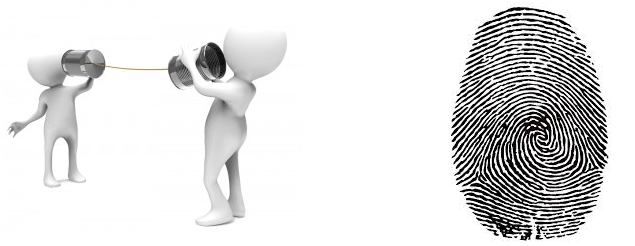
\includegraphics[width=0.8\columnwidth]{slide/coisa} 
  \caption{Baseada em \cite{Barrett}} 
  \label{fig:coisa}
\end{figure}
\end{frame}	

\begin{frame}{Internet das Coisas (IoT)}
\justifying
Rede mundial de objetos (coisas) unicamente endereçáveis e interconectados, seguindo os protocolos dos padrões de comunicação \cite{iot2020:2008}.
\begin{figure}[!htb] \centering 
  \centering
  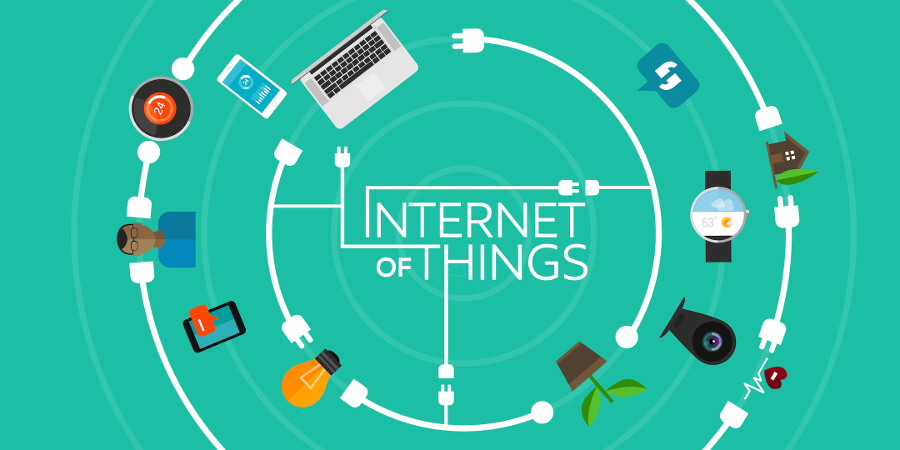
\includegraphics[width=.8\columnwidth]{slide/iot} 
  \caption{\footnote[frame]{\url{http://intca.org/2016/08/internet-of-things/}}} 
  \label{fig:iot}
\end{figure}
\end{frame}

\begin{frame}{Internet das Coisas (IoT)}
\justifying
Devido ao crescente número de coisas sendo conectadas, surgem diversos desafios, a exemplo de:
  \begin{itemize}
\justifying
    \item<1 -> Disponibilidade de uma interface de comunicação (acesso aos serviços e informações dos dispositivos) comum aos objetos.
    \item<2 -> Detecção e resolução de efeitos colaterais indesejáveis.
  \end{itemize}
\end{frame}

\begin{frame}{Desafios IoT: interface de comunicação padrão}
\justifying
Disponibilização das coisas como serviços Web RESTFul.
  \begin{itemize}
\justifying
    \item Mais leve que os serviços Web baseados em SOAP.
  \end{itemize}
\begin{figure}[!htb] \centering 
  \centering
  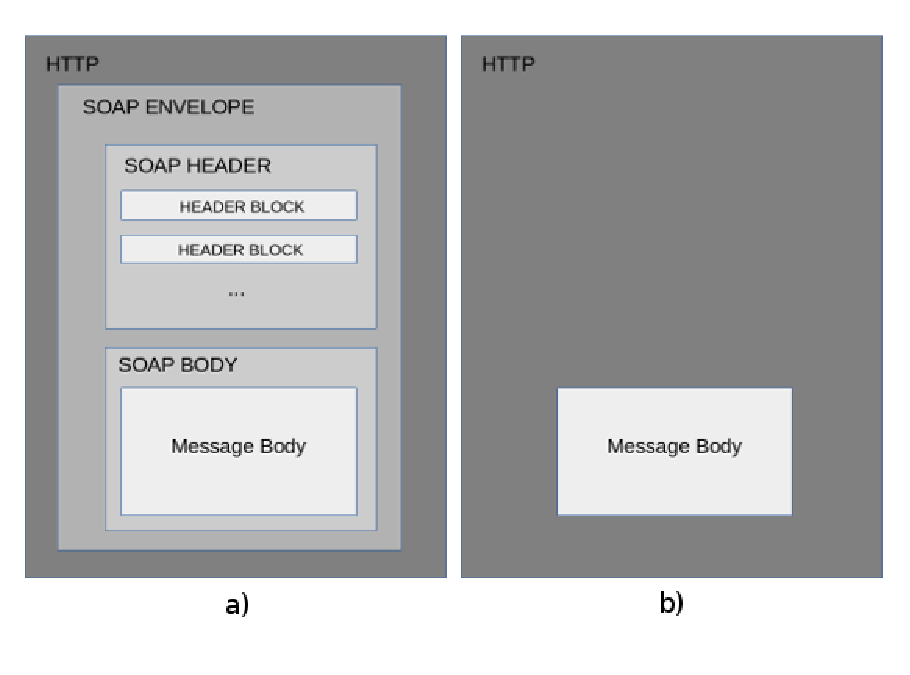
\includegraphics[width=.7\columnwidth]{slide/messages_restXsoap} 
  \caption{Baseada em \cite{Pautasso:2014}} 
  \label{fig:messages_restXsoap}
\end{figure}
\end{frame}

\begin{frame}{Desafios IoT: interface de comunicação padrão}
\justifying
Disponibilização das coisas como serviços Web RESTFul.
  \begin{itemize}
\justifying
    \item <1 ->Diferentes representações de um mesmo recurso (aumenta a interoperabilidade)
   \begin{examples}<1 ->
       JSON, XML, TEXT, TEXT\_HTML.
   \end{examples}
    \item <2 - >Interface com semântica bem definida.
   \begin{examples}<1 ->
          Utilização dos métodos HTTP (GET, PUT, DELETE, POST, HEAD, OPTIONS, dentre outros).
   \end{examples}
  \end{itemize}
\end{frame}

\begin{frame}{Desafios IoT: detecção e resolução de efeitos colaterais indesejáveis}
\justifying
Em desenvolvimento de \textit{software}, uma \alert{\textit{feature} (característica)} é um componente de adicional funcionalidade ao \textit{software} \cite{Calder:2003}, consistindo de um conjunto de requisitos logicamente relacionados e suas especificações, o qual se destina a fornecer um determinado efeito comportamental \cite{NHLABATSI:2008}.
\end{frame}

\begin{frame}{Desafios IoT: detecção e resolução de efeitos colaterais indesejáveis}
\justifying
Quando a \alert{composição de \textit{features}} leva a algum \alert{comportamento não esperado} - interação de características, esta pode resultar em \alert{efeitos colaterais indesejáveis}: um estado inconsistente do sistema, um sistema instável ou dados imprecisos \cite{NHLABATSI:2008}.
\end{frame}


\section{Proposta}
\begin{frame}{Proposta}
\justifying
Detectar efeitos colaterais indesejáveis de uma maneira inteligente, utilizando o método \textit{ensemble} DECORATE, no cenário ``Levar compras'' do \textit{Home Network System} (HNS).
\end{frame}

\begin{frame}{HNS}
Rede doméstica de coisas (aparelhos domésticos e sensores) com capacidade de conectividade de rede e, interface de controle e monitoramento. Os dispositivos da casa são compostos uns com os outros para prover funcionalidades que atendam aos requisitos dos usuários da casa \cite{Ikegami:2013}.
\end{frame}

\begin{frame}{HNS do Cenário Levar compras}
\begin{figure}[!htb] \centering 
  \centering
  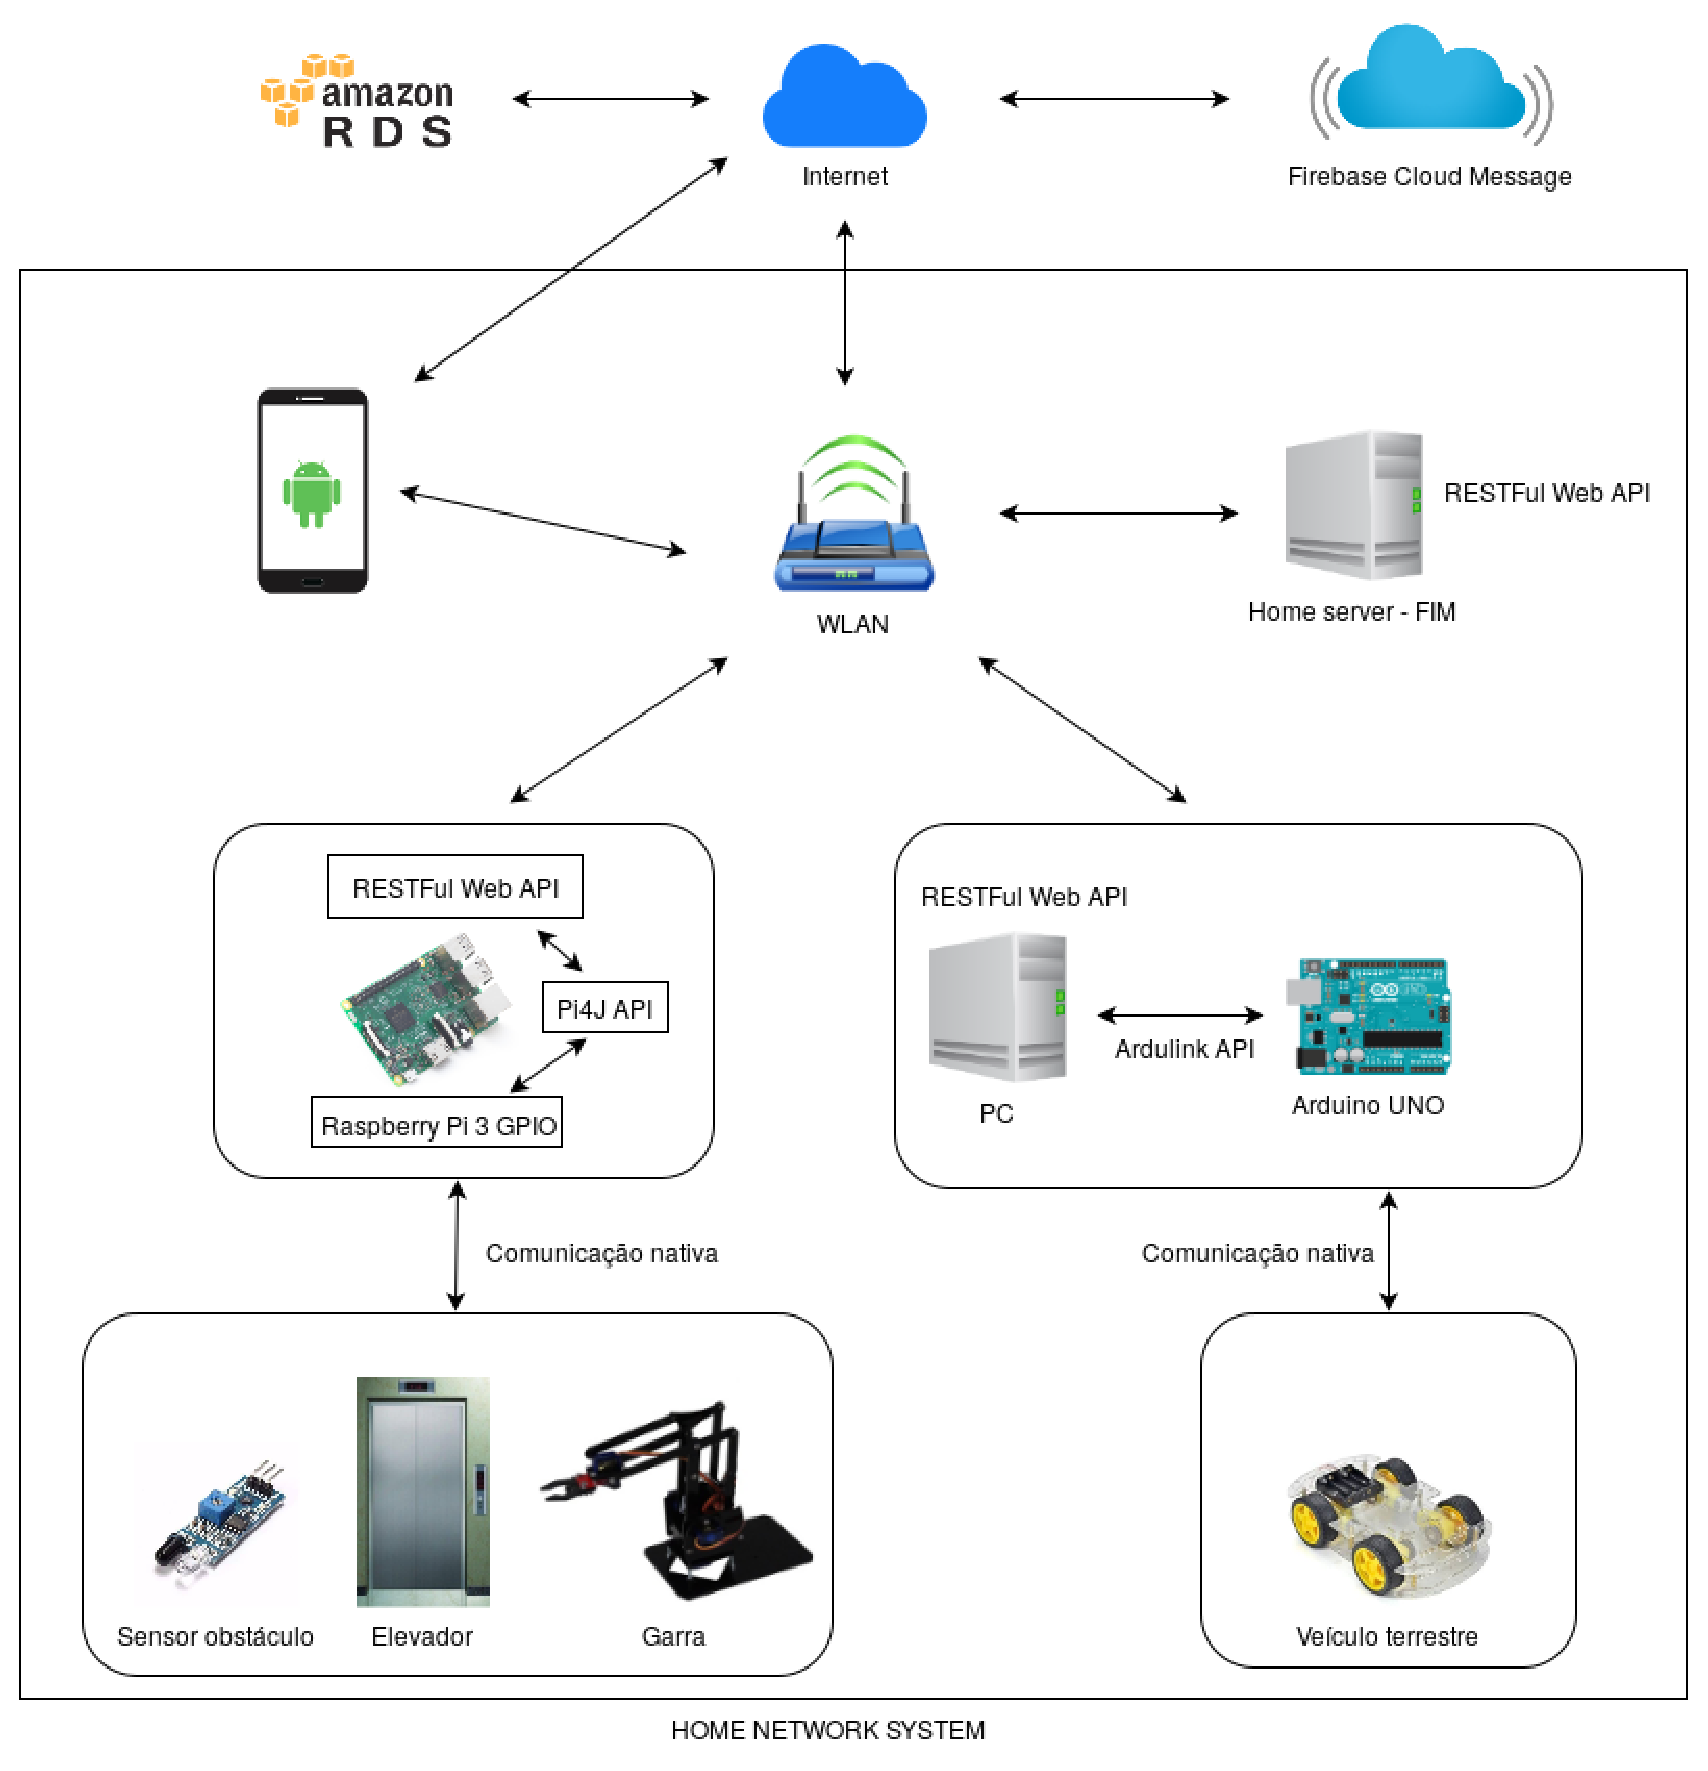
\includegraphics[width=0.7\columnwidth]{slide/cenario} 
  \caption{Cenário Levar compras.} 
  \label{fig:hns}
\end{figure}
\end{frame}


\subsection{Cenário Levar compras}
\begin{frame}{Objetos das compras (cestas)}
\begin{figure}[!htb] \centering 
  \centering
  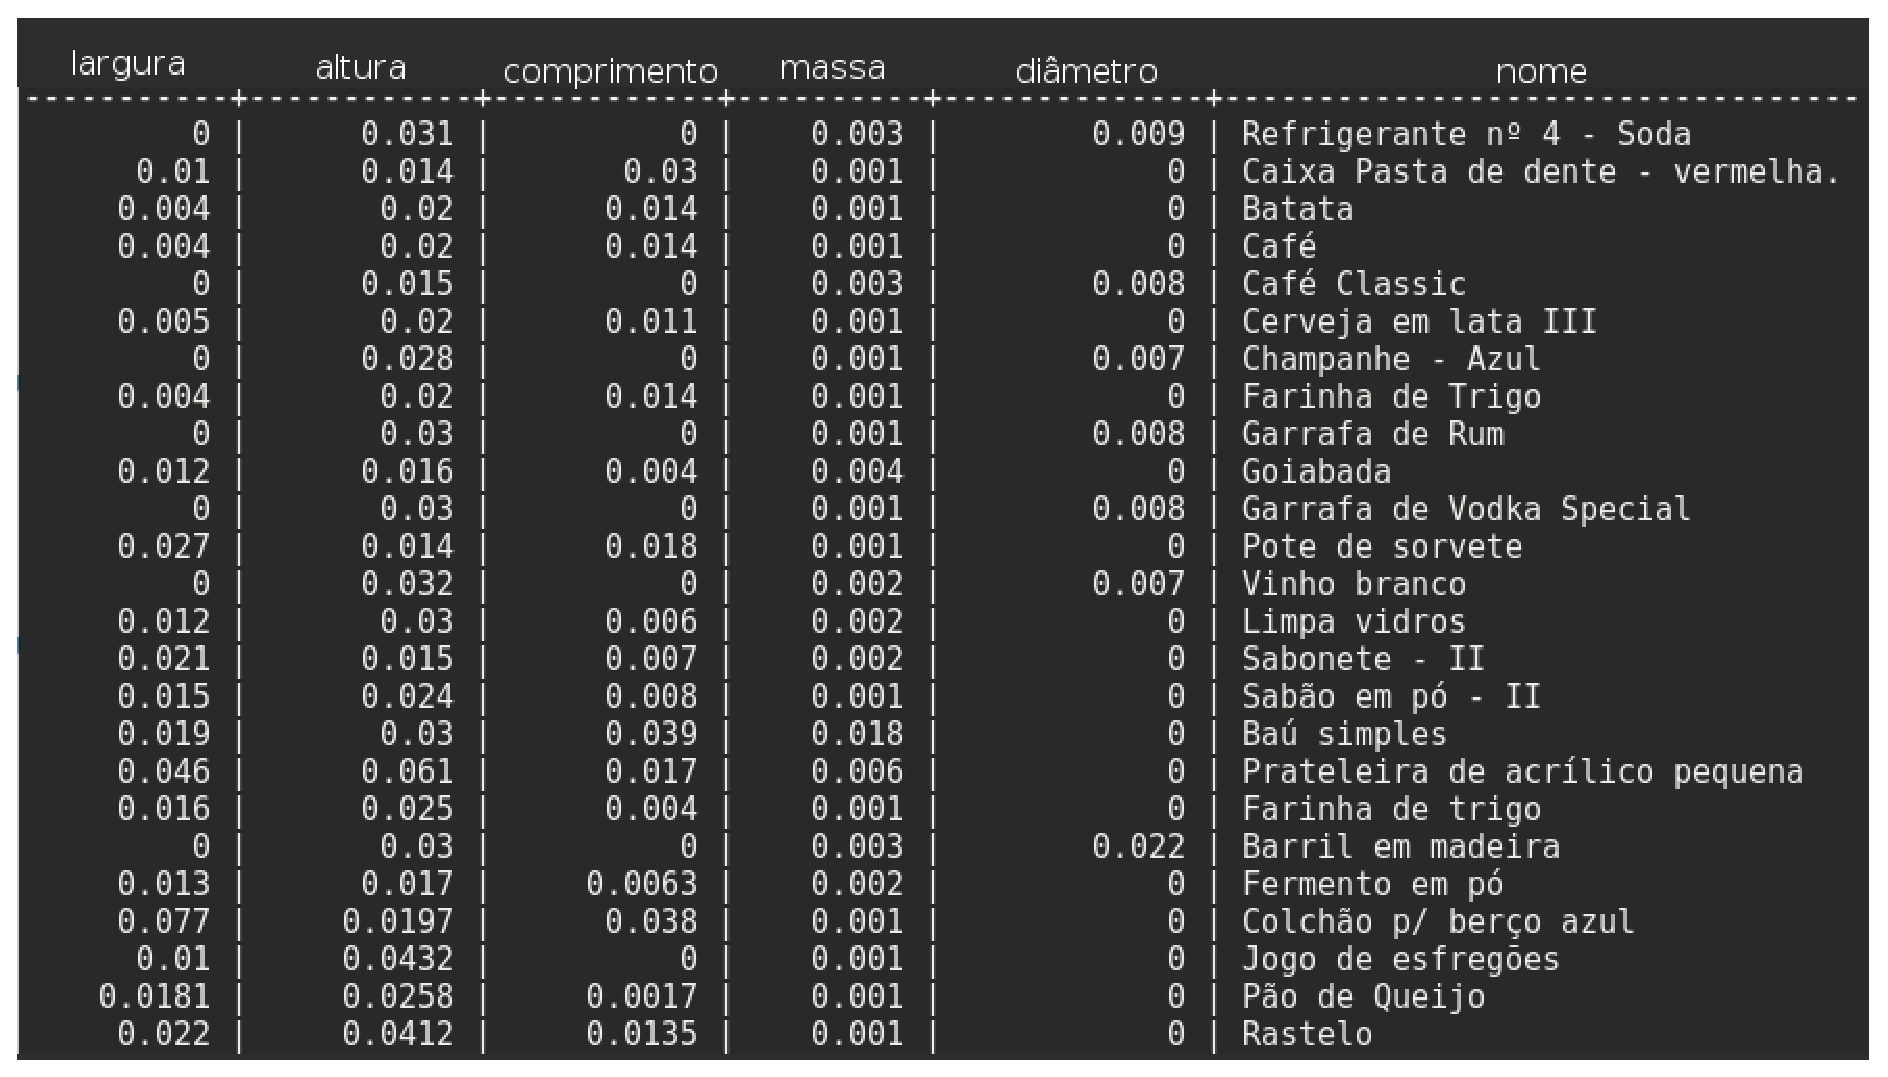
\includegraphics[width=0.9\columnwidth]{slide/lista_items} 
  \caption{Objetos das compras (cestas). Medidas em metros (m).} 
  \label{fig:lista_items}
\end{figure}
\end{frame}

\begin{frame}{Exemplos de Compras (cestas)}
\begin{figure}[!htb] \centering 
  \centering
  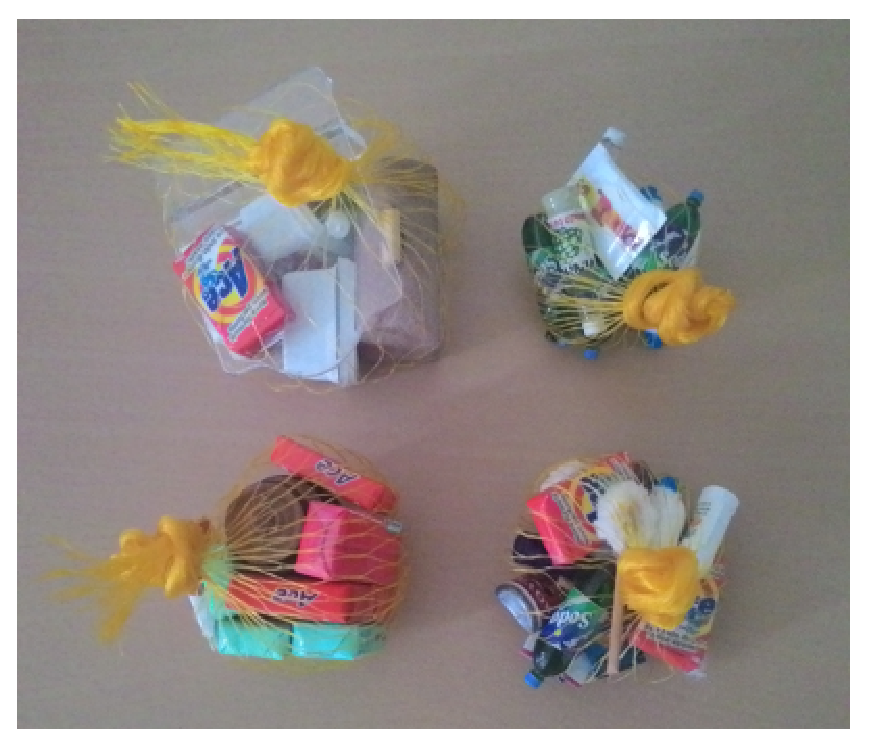
\includegraphics[width=0.7\columnwidth]{slide/exemplos_cesta} 
  \caption{Exemplos de cestas.} 
  \label{fig:exemplos_cesta}
\end{figure}
\end{frame}

\begin{frame}{Cenário Levar compras}
\begin{figure}[!htb] \centering 
  \centering
  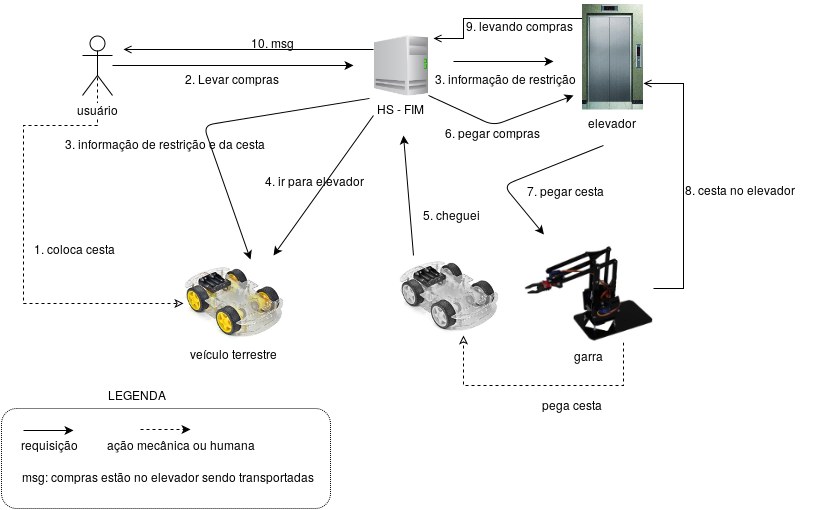
\includegraphics[width=0.9\columnwidth]{slide/cenario_requests} 
  \caption{Cenário Levar compras.} 
  \label{fig:cenariolevarcompras}
\end{figure}
\end{frame}


\subsection{Método de detecção}
\subsubsection{Geração da massa de dados}
\begin{frame}{Geração da massa de dados}
   \begin{itemize}
\justifying
      \item <1 ->Confeccionadas 59 cestas.
      \item <2 ->Verificado se as cestas cabiam dentro do elevador.
      \item <3 ->Registro no banco de dados relacional na nuvem.
      \item <4 ->Cenário Levar compras executado 59 vezes.
   \end{itemize}
\end{frame}

\begin{frame}{Geração da massa de dados}
   \begin{itemize}
\justifying
      \item <1 ->Algumas vezes o comportamento da garra fazia com que a cesta não ficasse corretamente no compartimento do elevador, impedindo o elevador continuar com a funcionalidade ``Levar compras''. Provocando um \alert{efeito colateral indesejável}.
      \item <2 ->Cada cesta foi rotulada como \alert{``É efeito colateral''} ou \alert{``não é éfeito colateral''} e atualizado valor no banco.
   \end{itemize}
\end{frame}


\subsubsection{Seleção dos atributos}
\begin{frame}{Seleção dos atributos}
   \begin{itemize}
\justifying
      \item <1 ->Uma cesta com 10 objetos tem \alert{$10 \times 5=50$ atributos}.
      \item <2 ->Usado os valores das médias e totais da medidas, assim como a quantidade de objetos. Reduzindo a \alert{11 atributos}.
   \end{itemize}
\end{frame}

\begin{frame}{Seleção dos atributos}
   \begin{itemize}
\justifying
      \item <1 ->Construído arquivo ``arff'', padrão WEKA \cite{Hall:2009}, com 59 instâncias.
      \item <2 ->Cada instância representa uma cesta com 11 parâmetros numéricos mais 1 nominal.
      \item <3 -> Gerou-se uma visualização do espaço de atributos em 2D, ou seja, par a par.
   \end{itemize}
\end{frame}

\begin{frame}{Seleção dos atributos}
\begin{figure}[!htb] \centering 
  \centering
  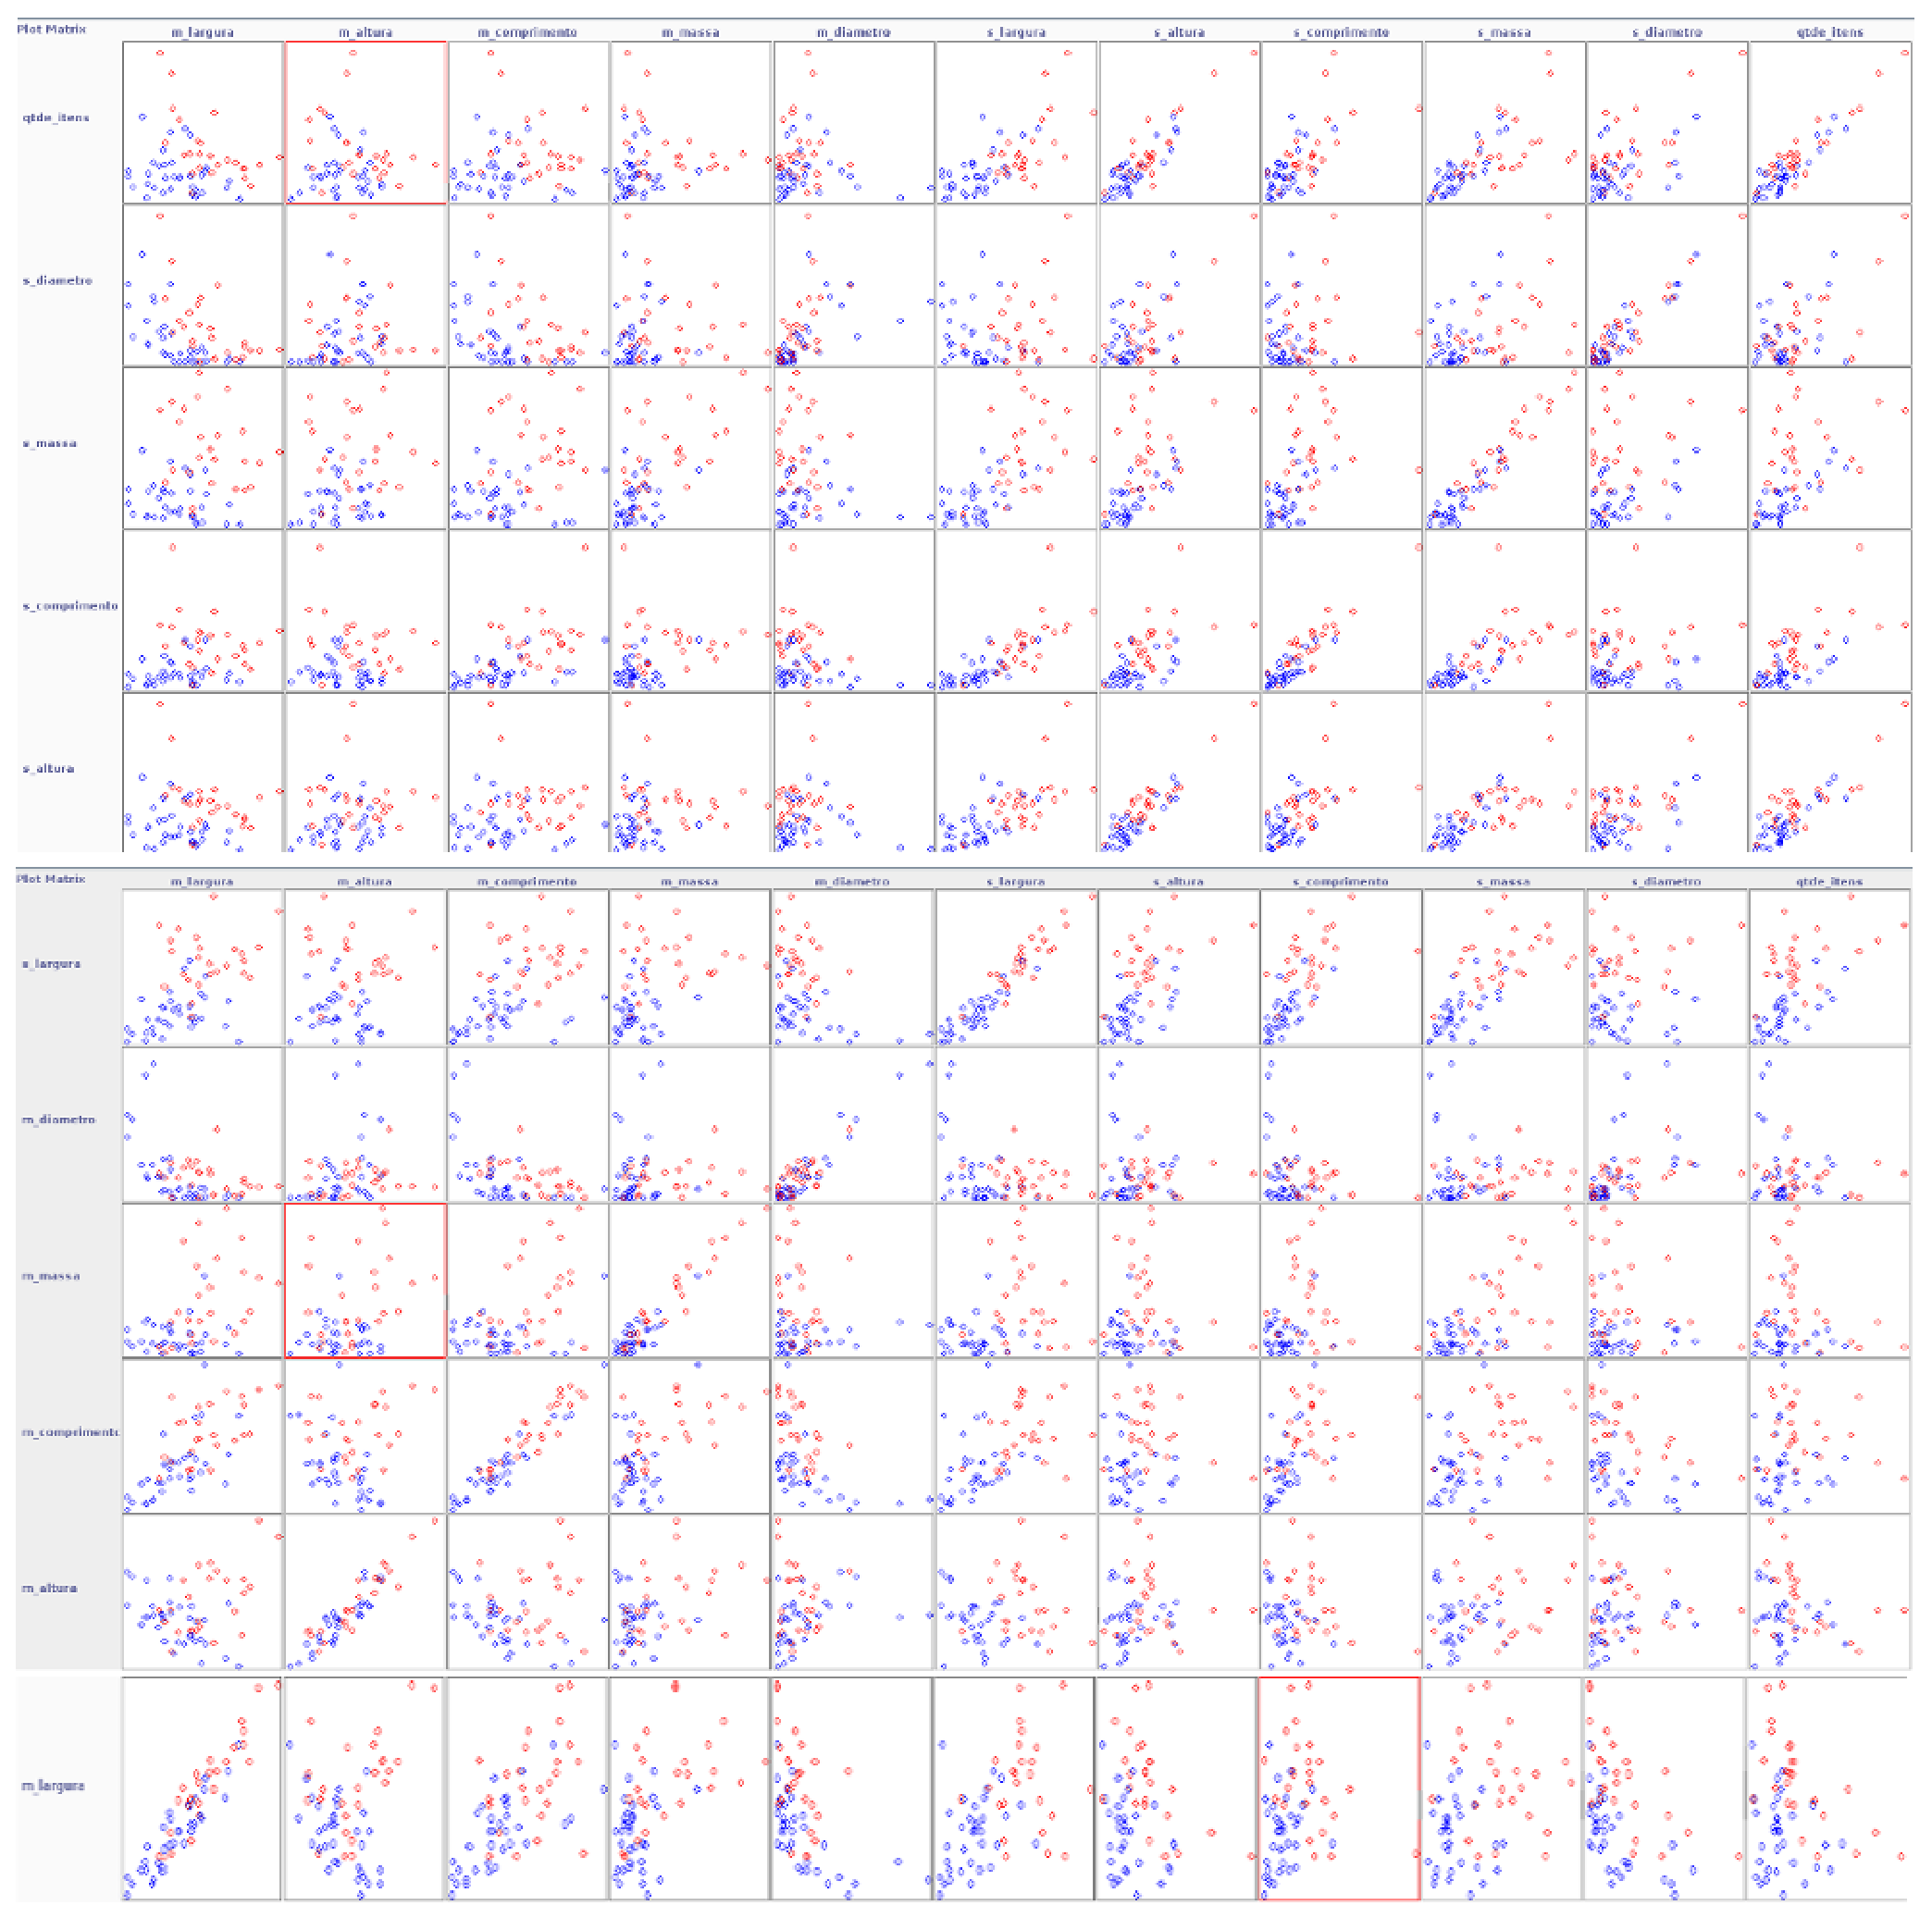
\includegraphics[width=0.7\columnwidth]{slide/all_plot} 
  \caption{Espaço de atributos em 2D.} 
  \label{fig:all_plot}
\end{figure}
\end{frame}

\begin{frame}{Seleção dos atributos - 3 pares selecionados}
\begin{figure}[!htb] \centering 
  \centering
  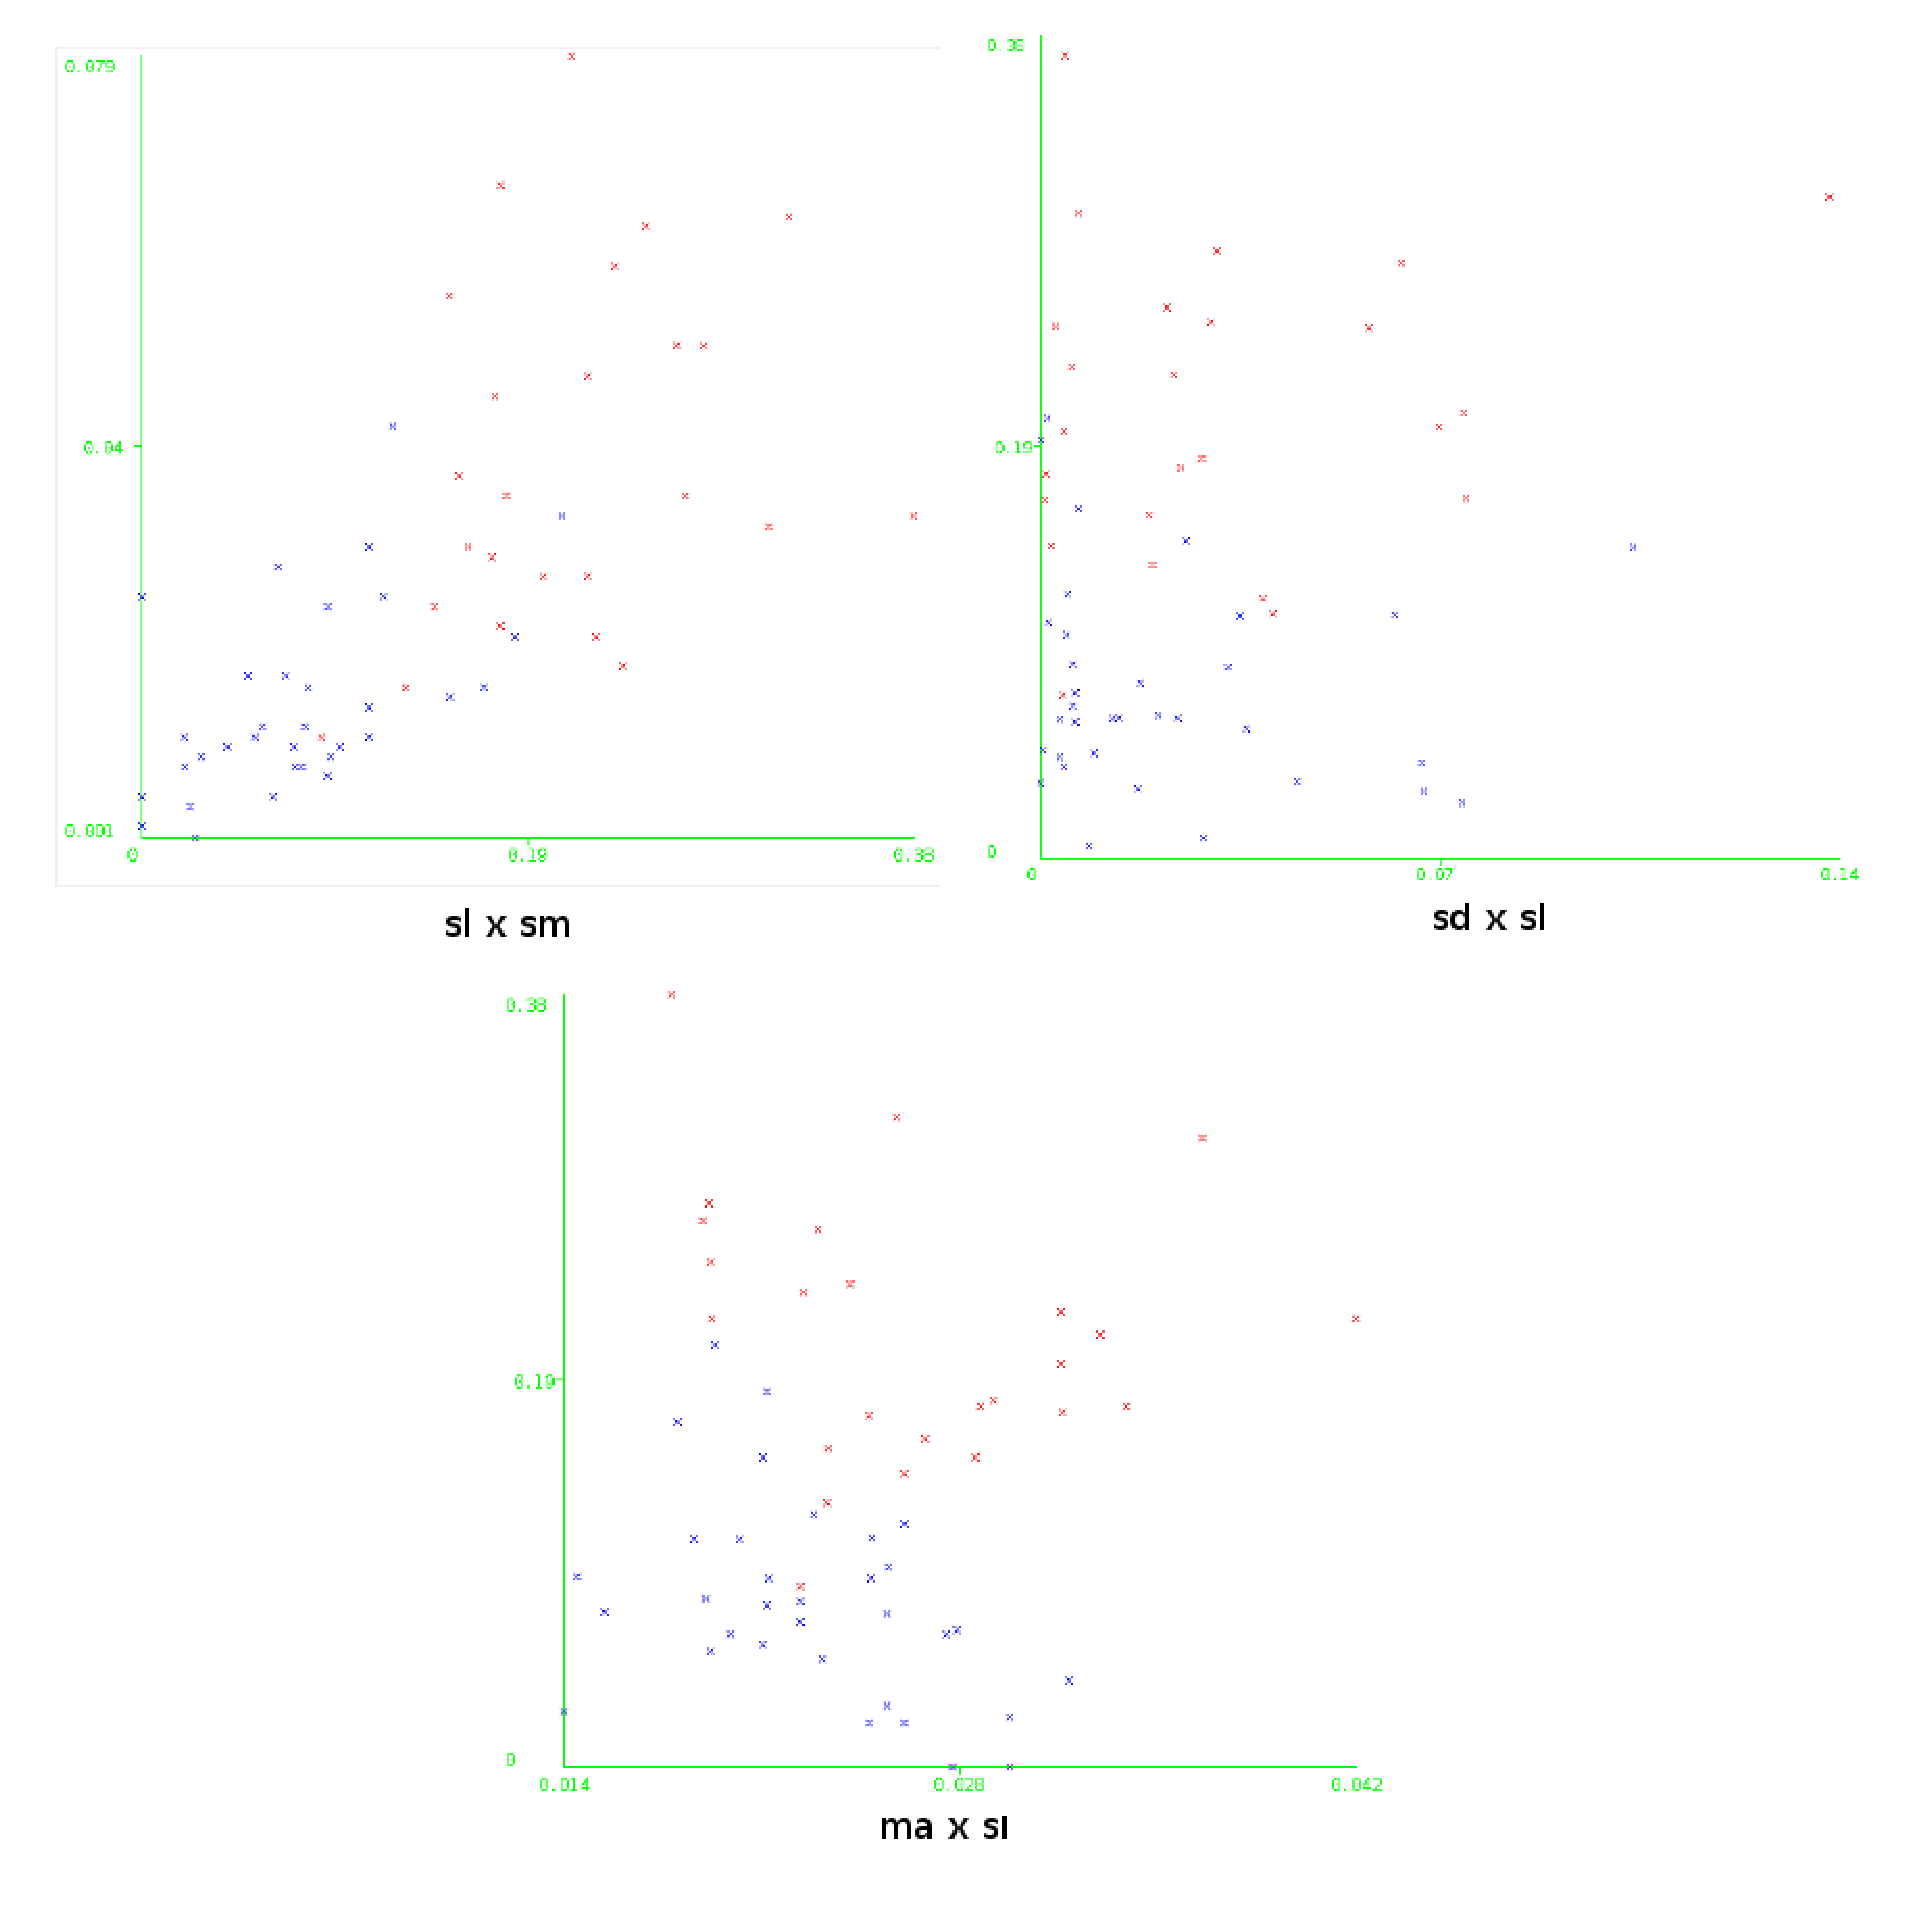
\includegraphics[width=0.7\columnwidth]{slide/eixos_4_atributos} 
  \caption{Separação das classes entre os atributos (somaLargura, somaMassa) - ``sl x sm'', (somaDiâmetro, somaLargura) - ``sd x sl'' e, (médiaAltura, somaLargura).} 
  \label{fig:eixos_4_atributos}
\end{figure}
\end{frame}


\subsubsection{Método ensemble DECORATE }

\begin{frame}{DECORATE \cite{Melville:2003, Melville:2004, *}}
\justifying DECORATE (Diverse Ensemble Creation by Oppositional Relabeling of Artificial Training Examples).
   \begin{itemize}
\justifying
      \item Combina o resultado de diversos classificadores para chegar em uma decisão final.
   \end{itemize}

\begin{equation}
  P_{y}(x) = \frac{\sum\limits_{C_{i}\in C^*} P_{C_{i,y}}(x)}{|C^*|}
  \label{eq:decorate}
\end{equation}

%\begin{equation}
 % C^*(x) = \argmax_{y\in Y} P_{y}(x)
  %\label{eq:decorate}
%\end{equation}

\end{frame}

\begin{frame}{DECORATE}
   \begin{itemize}
\justifying
      \item Utiliza dados adicionais de treino gerados artificialmente.
   \end{itemize}
   \begin{figure}[!htb] \centering 
     \centering
     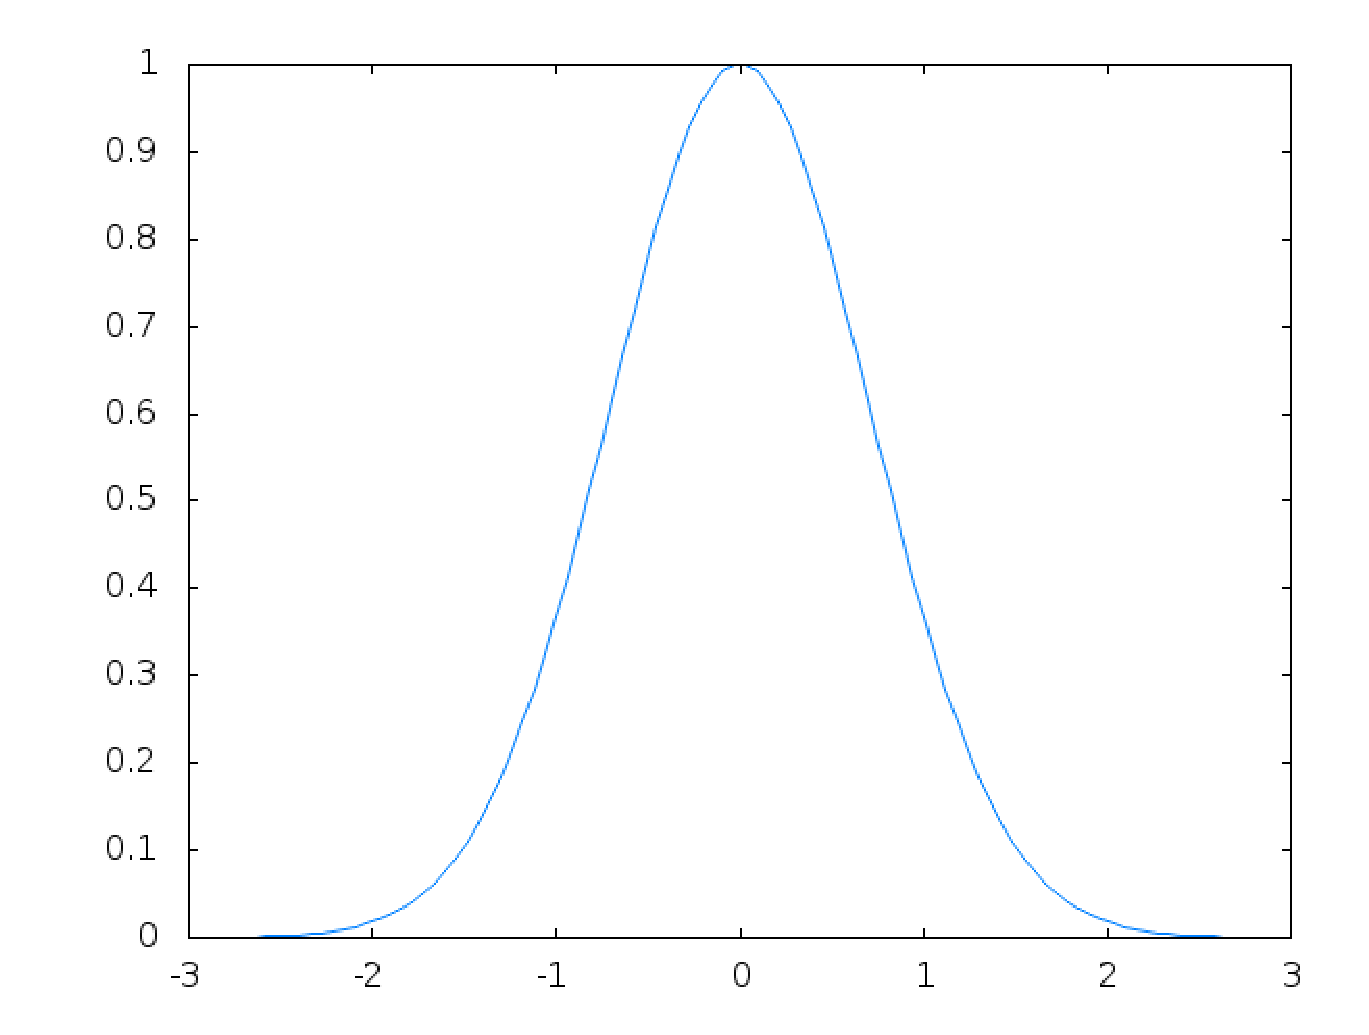
\includegraphics[width=.65\columnwidth]{slide/gaussiana1} 
     \caption{Curva Gaussiana. \footnote[frame]{\url{http://proooof.blogspot.com.br/2011/12/sigma.html}}} 
     \label{fig:gaussiana1}
   \end{figure}
\end{frame}

\begin{frame}{DECORATE}
   \begin{itemize}
\justifying
      \item Utiliza dados adicionais de treino gerados artificialmente.
\end{itemize}
      \begin{itemize}
\justifying
      \item <1 ->Primeiramente utiliza a probabilidade do \textit{ensemble} $P_y(x)$.
      \item <2 ->Por fim utiliza a expressão abaixo para rotular o exemplo artificial.
\begin{equation}
     P_{y}^{-1}(x) = \frac{\frac{1}{P_y(x)}}{\sum\limits_y \frac{1}{P_y(x)}}
     \label{eq:decorate}
   \end{equation}
   \end{itemize}
\end{frame}

\begin{frame}{DECORATE}
   \begin{figure}[!htb] \centering 
     \centering
     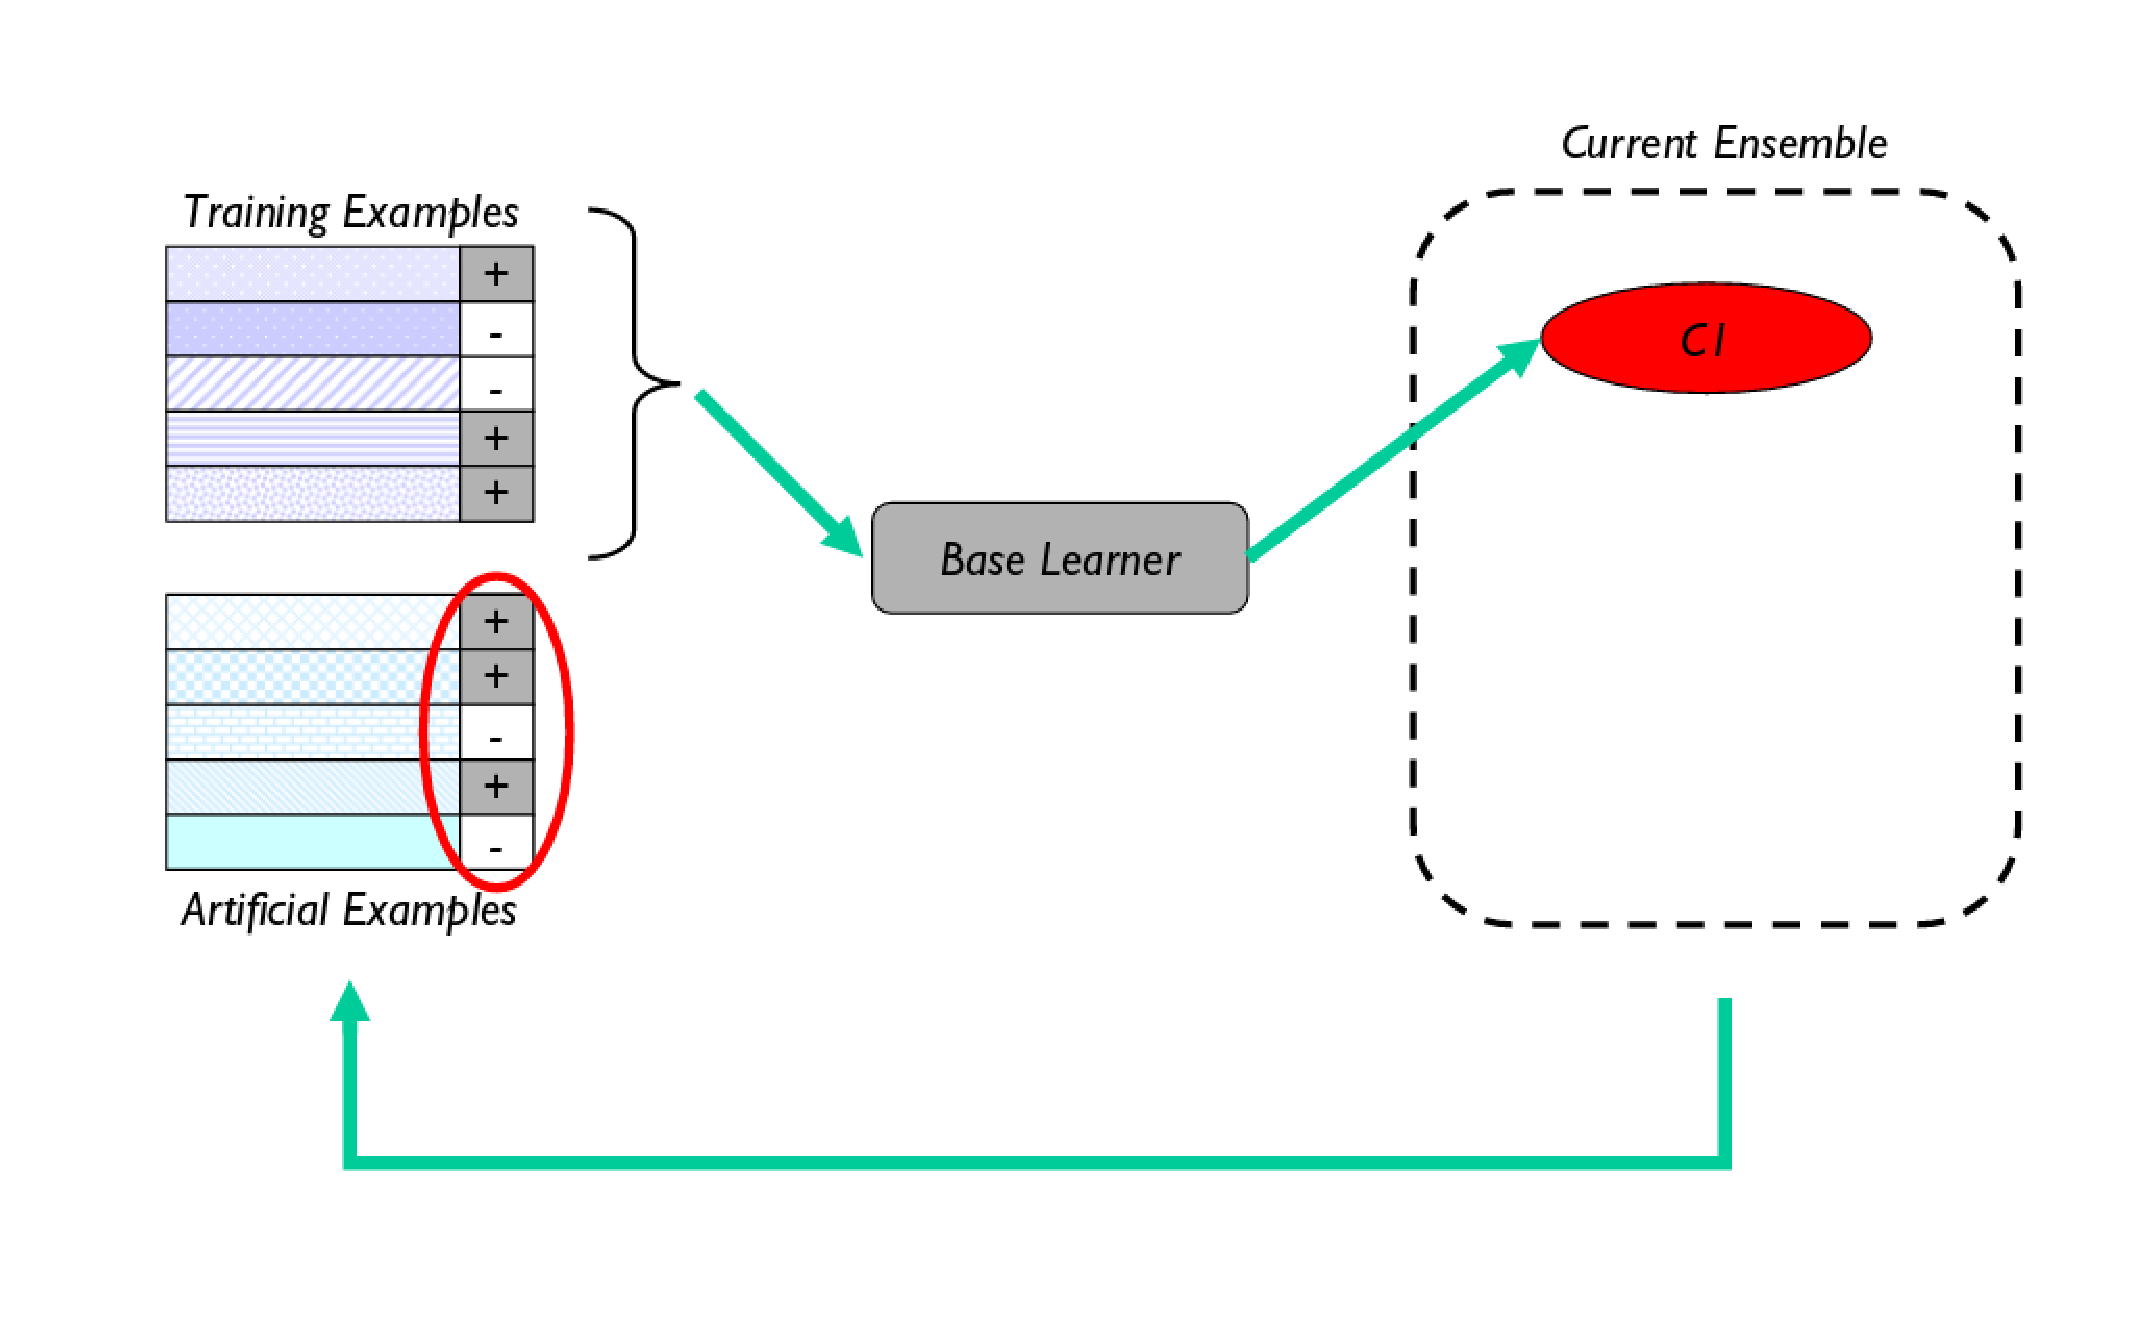
\includegraphics[width=.8\columnwidth]{slide/decorate1} 
     \caption{DECORATE 1ª iteração. \footnote[frame]{\url{http://www.time.mk/trajkovski/teaching/aim/Lecture8.pdf}}} 
     \label{fig:decorate1}
   \end{figure}
\end{frame}

\begin{frame}{DECORATE}
\begin{figure}[!htb] \centering 
  \centering
  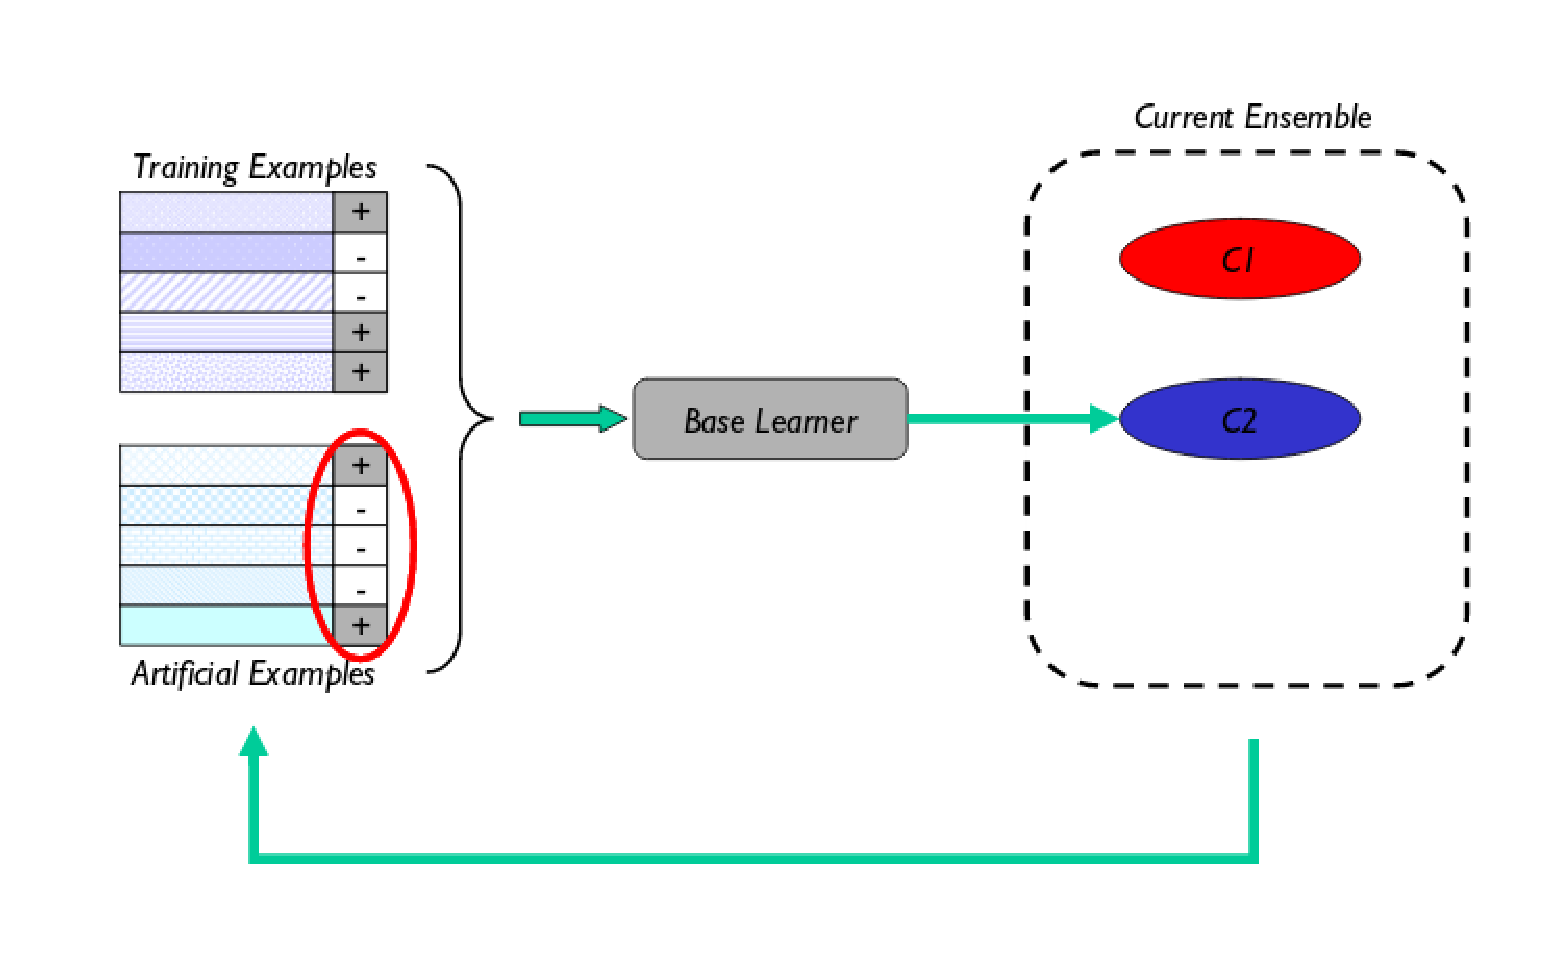
\includegraphics[width=.8\columnwidth]{slide/decorate2} 
  \caption{DECORATE 2ª iteração. \footnote[frame]{\url{http://www.time.mk/trajkovski/teaching/aim/Lecture8.pdf}}} 
  \label{fig:decorate2}
\end{figure}
\end{frame}

\begin{frame}{Parâmetros DECORATE \cite{Melville:2004}}
   \begin{itemize}
\justifying
      \item <1 ->Número máximo de iterações = 50.
      \item <2 ->Número máximo de classificadores = 14.
      \item <3 ->Classificador base = J48. 
      \item <4 ->Quantidade de exemplos artificiais = 100\% do \textit{dataset} de treino.
   \end{itemize}
\end{frame}


\subsection{Implantação do método proposto}
\begin{frame}{Implantação do método proposto}
\begin{figure}[!htb] \centering 
  \centering
  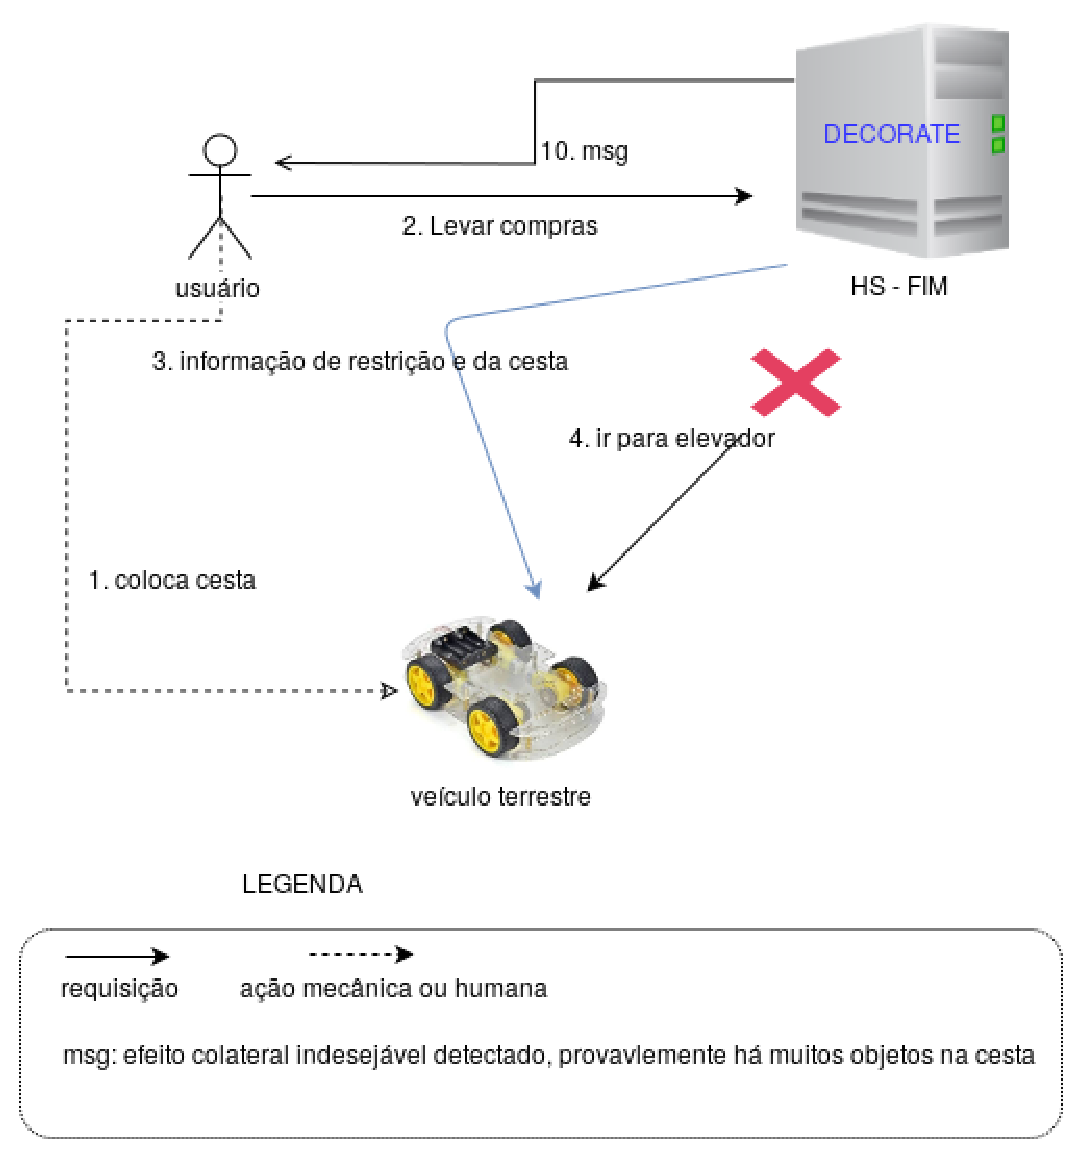
\includegraphics[width=0.6\columnwidth]{slide/cenario_deteccao} 
  \caption{Atuação do DECORATE no cenário Levar compras.} 
  \label{fig:cenario_deteccao}
\end{figure}
\end{frame}


\section{Validação}
\begin{frame}{TP, TN, FP, FN \cite{Olson:2008}}
   \begin{itemize}
      \item <1 ->Verdadeiro positivo (TP): instância que pertence a classe positiva e que foi corretamente classificada como positiva.
      \item <2 ->Verdadeiro negativo (TN): instância que pertence a classe negativa e que foi classificada corretamente como negativa.
      \item <3 ->Falso positivo (FP): instância que pertence a classe negativa e que foi classificada  incorretamente como positiva.
      \item <4 ->Falso negativo (FN): instância que pertence a classe positiva e que foi classificada incorretamente como negativa.
\justifying
   \end{itemize}
\end{frame}

\begin{frame}{Accuracy \cite{Metz:1978}}
   \begin{itemize}
\justifying
     \item \textit{Accuracy}: taxa correta de classificação em relação a todos os exemplos. 
   \end{itemize}
\vspace{0.3in}
\begin{equation} 
  Accuracy = \frac{TP+TN}{TP+TN+FP+FN} 
  \label{eq:accuracy}
\end{equation}
\end{frame}

\begin{frame}{Precision, Recall \cite{Davis:2006}}
   \begin{itemize}

      \item <1 ->\textit{Precision}: Dentre todos os exemplos classificados como positivos, quais realmente são positivos ? 
\justifying
\begin{equation} 
  Precision = \frac{TP}{TP+FP}
  \label{eq:precision}
\end{equation}

      \item <2 ->\textit{Recall} ou \textit{True Positive Rate - TPR}: Dentre os exemplos classificados como positivos (que realmente são positivos) e os classificados como negativos (mas que são positivos), qual a taxa de exemplos positivos classificados corretamente?

\begin{equation} 
  Recall = \frac{TP}{TP+FN} 
  \label{eq:recall}
\end{equation}

   \end{itemize}
\end{frame}


\subsection{Método avaliativo stratified-k-fold-cross-validation}
\begin{frame}{stratified-k-fold-cross-validation}
\begin{figure}[!htb] \centering 
  \centering
  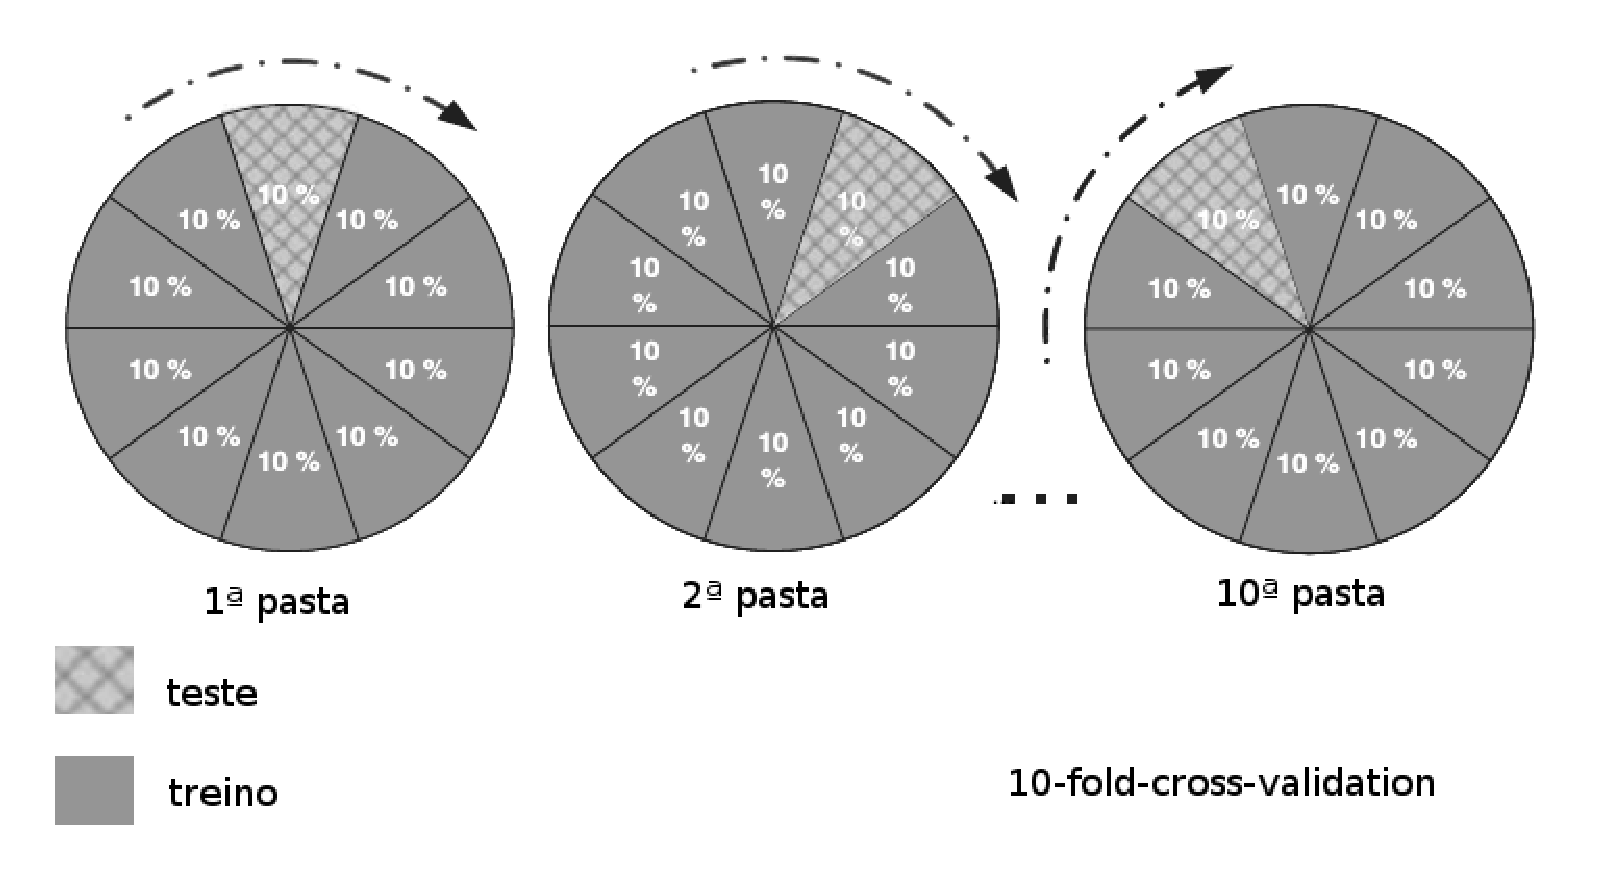
\includegraphics[width=0.8\columnwidth]{slide/k-fold-crossvalidation} 
  \caption{k-fold-cross-validation. Adaptado de \cite{Olson:2008}.} 
  \label{fig:k-fold-crossvalidation}
\end{figure}
\end{frame}

\subsection{Experimentos}
\begin{frame}{Experimentos}
   \begin{itemize}
\justifying
      \item <1 ->Para cada par de atributos selecionados utilizou-se \textit{stratified-10-fold-cross-validation} (repetido dez vezes) juntamente com o \textit{ensemble DECORATE} a fim de verificar se é possível generalizar pelo menos um modelo.
      \item <2 ->Em cada verificação construiu-se um modelo com diferentes frações do dataset, variando de 16 instâncias a 59 instâncias e, construiu-se uma curva de aprendizado.
      \item <3 ->Selecionou-se a curva que mais crescia e se mantia regular e, com melhor taxa de \textit{recall}.
      \item <4 ->Verificou a partir de que ponto esta curva tinha os melhores valores de \textit{recall}, \textit{precision} e \textit{accuracy}.
      \item <5 ->Realizou um procedimento de geração de modelo final a partir desse melhor ponto.
   \end{itemize}
\end{frame}


\subsection{Resultados e discussão}
\subsubsection{Modelos}
\begin{frame}{Resultados: $10\times$stratified-10-fold-cross-validation}
\begin{figure}[!htb] \centering 
  \centering
  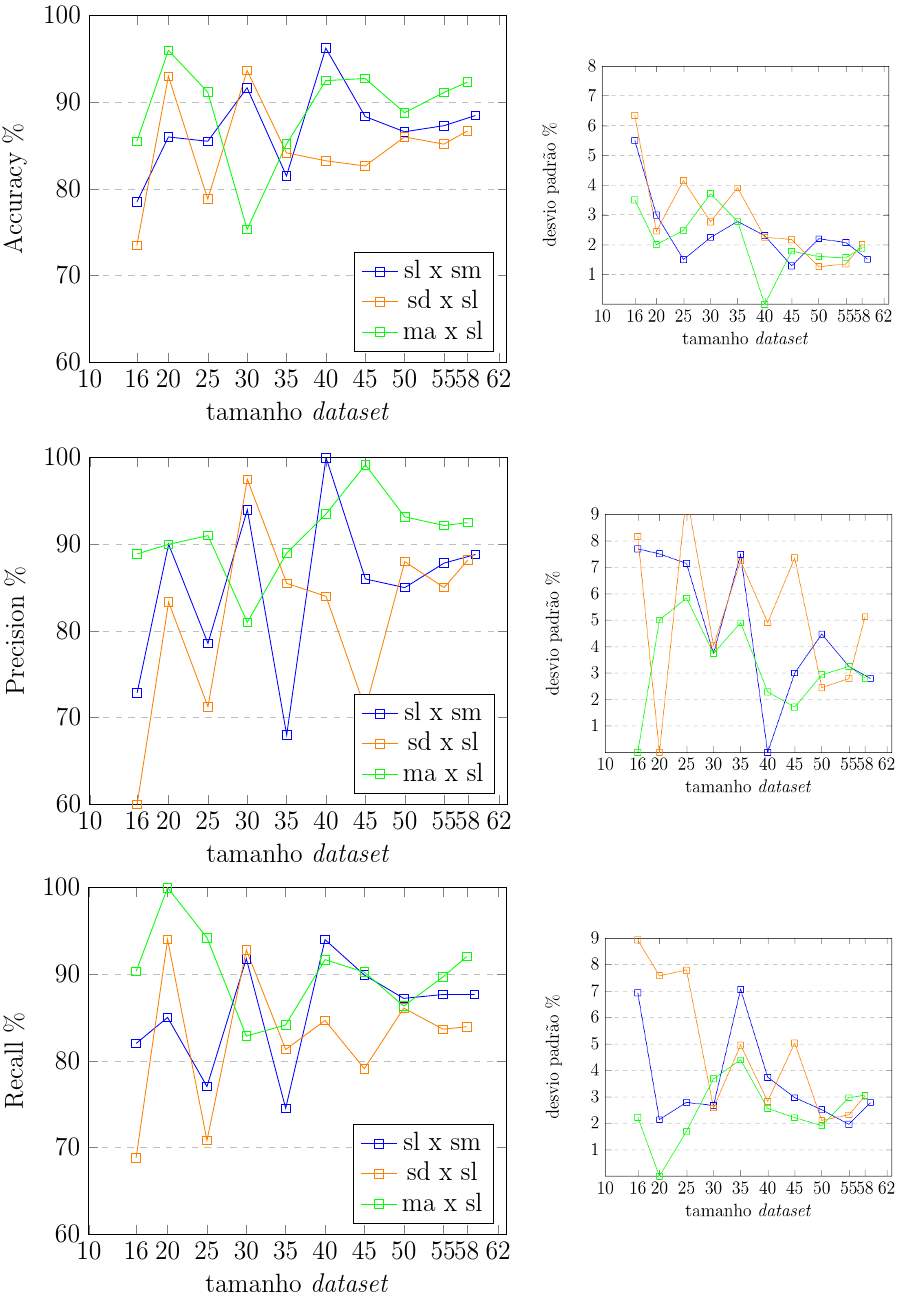
\includegraphics[width=0.5\columnwidth]{slide/accuracy_precision_recall} 
  \caption{} 
  \label{fig:accuracy_precision_recall}
\end{figure}
\end{frame}

\begin{frame}{Resultados: curva de aprendizado selecionada}
   \begin{table}[!htp]
      \centering
      \resizebox{0.75\textwidth}{!}{\begin{minipage}{\textwidth}
     \begin{tabular}{ |l|c c c c c|}
       \hline
          {\bf \textbf{$n^o i$}} & {\bf 40} & {\bf 45} & {\bf 50} & {\bf 55} & {\bf 58} \\
       \hline
          \textbf{A, DP} & 92.5, 0 & 92.75, 1.78 & 88.8, 1.6 & 91.13, 1.56 & 92.33, 1.89 \\
       \hline
          \textbf{P, DP} & 93.5, 2.29 & 99.17, 1.71 & 93.17, 2.93 &  92.17, 3.25 & 92.5, 2.81 \\
       \hline
          \textbf{R, DP} & 91.69, 2.56 & 90.25, 2.21 & 86.33, 1.91 & 89.71, 2.97 & 92.05, 3.06 \\
       \hline
     \end{tabular}
     \label{table:valorescurva}
   \end{minipage}}
      \caption{\justifying Valores das curvas ``ma x sl'' da Figura \ref{fig:accuracy_precision_recall} a partir do \textit{dataset} com 40 instâncias. A (\textit{Accuracy}), P (\textit{Precision}, R (\textit{Recall}), DP (Desvio Padrão), i (instâncias). Os valores A, P, R e DV estão em \%.}
   \end{table}

\resizebox{0.85\textwidth}{!}{\begin{minipage}{\textwidth}
   \begin{equation}
     (\textit{accuracy} \geq (92.75-1.78)) \wedge (\textit{precision} \geq (99.17-1.71)) \wedge (\textit{recall} \geq 90.25)
     \label{eq:esxpvalclass}
   \end{equation}
\end{minipage}}

\end{frame}

\begin{frame}{Resultados: geração do modelo final}
   \begin{figure}[!htb] \centering 
     \centering
     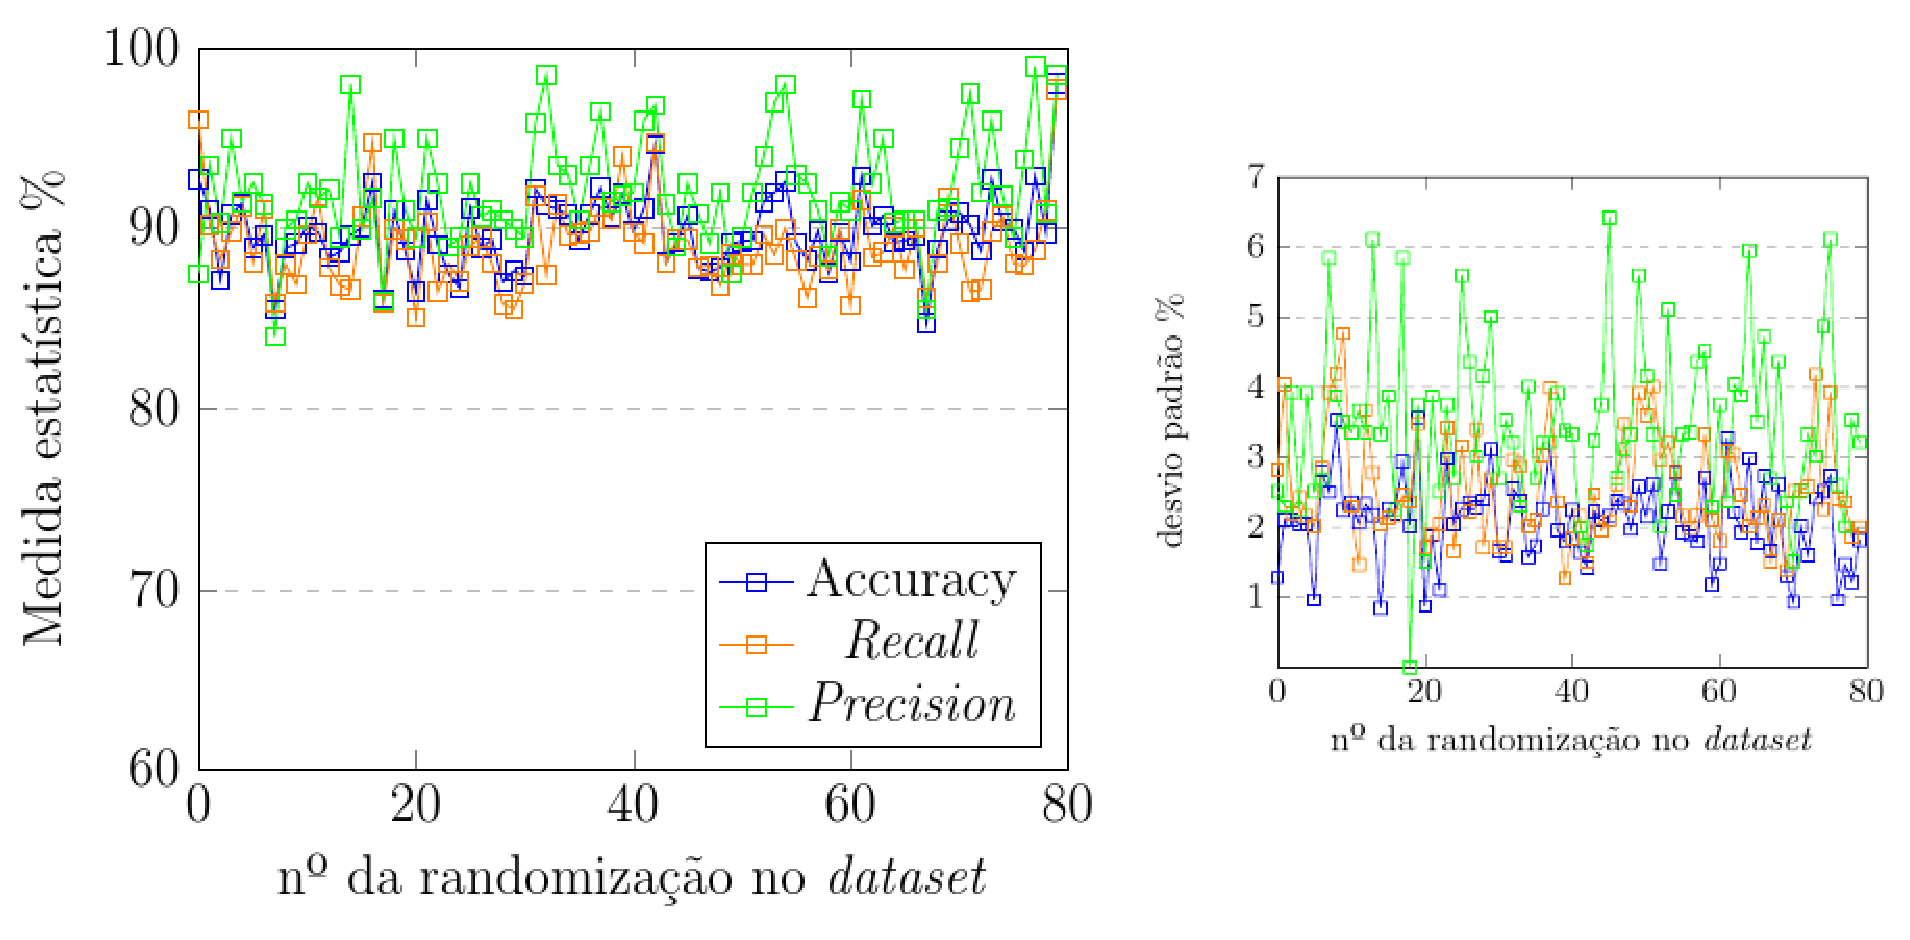
\includegraphics[width=1.0\columnwidth]{slide/apr45_dev} 
     \caption{\justifying \textit{stratified-10-fold-cross-validation} (repetido dez vezes). 45 instâncias foram escolhidas randomicamente em cima do \textit{dataset} de 59 instâncias. Procedimento repetido até que satisfizesse a expressão \ref{eq:esxpvalclass}. } 
     \label{fig:apr45_dev}
   \end{figure}
\end{frame}

\begin{frame}{Resultados: geração do modelo final}
\begin{table}[!htp]
  \centering
  \begin{tabular}{ |l|c|c|}
    \hline
       {\bf } & {\bf } & {\bf Desvio Padrão \%} \\
    \hline
       \textbf{Accuracy} \% & 98.05 & 1.81 \\
    \hline
       \textbf{Precision} \% & 98.5 & 3.2 \\
    \hline
       \textbf{\textit{Recall} \%} & 97.67 & 2 \\
    \hline
  \end{tabular}
  \caption{Valores da validação do modelo final.}
  \label{table:valmodelfinal}
\end{table}
\end{frame}


\subsubsection{Implantação}
\begin{frame}{Resultados: Implantação do modelo final}
   \begin{figure}[!htb] \centering 
     \centering
     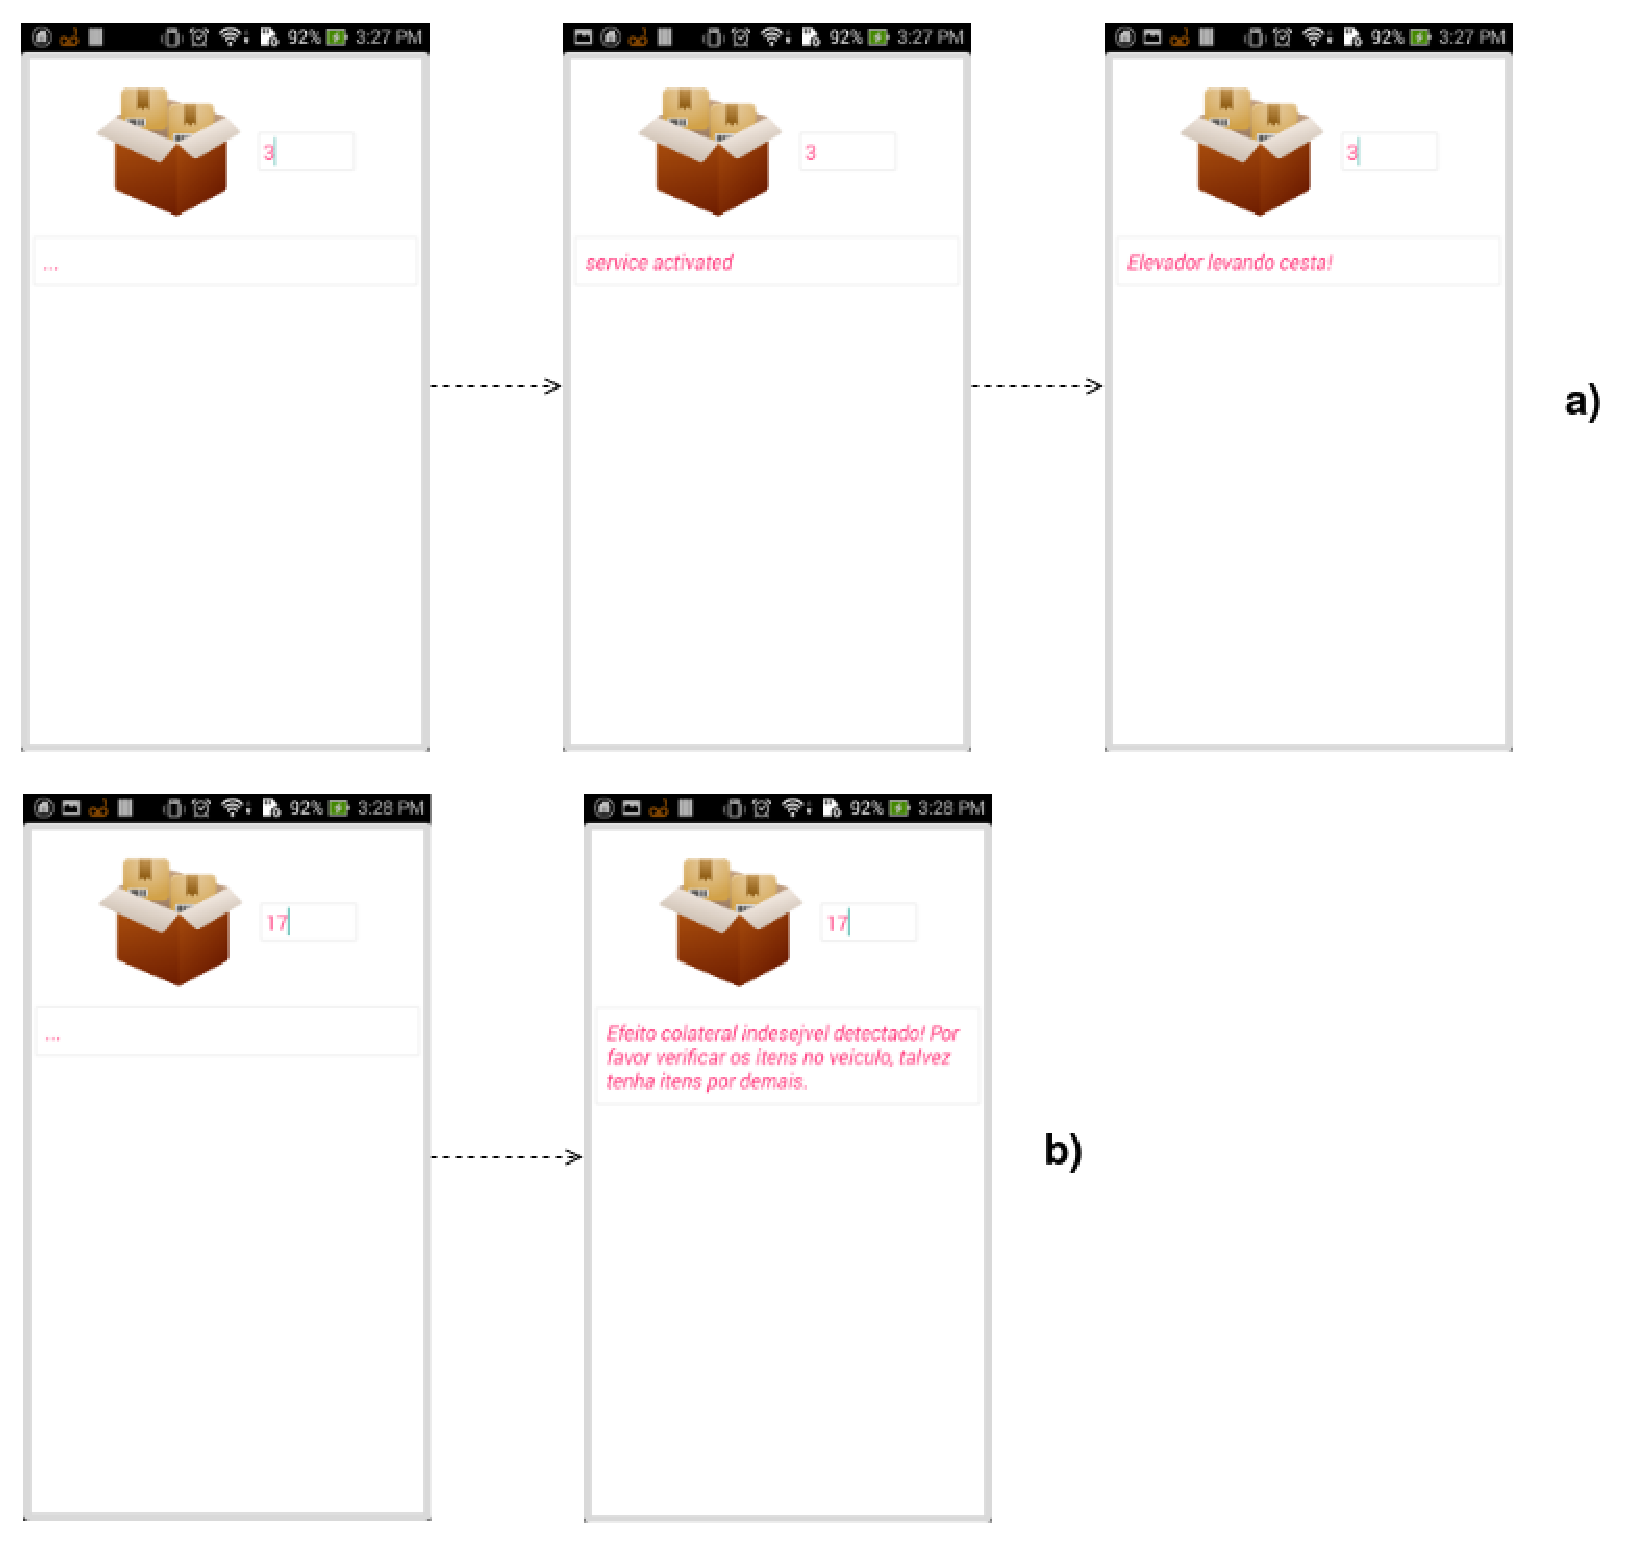
\includegraphics[width=.75\columnwidth]{slide/deteccao_efeito} 
     \caption{ \justifying Modelo classificatório atuando no cenário ``Levar compras'' do FIM. a) Fluxo da aplicação sem efeito colateral indesejável. b) Fluxo da aplicação com efeito colateral indesejável.} 
     \label{fig:deteccao_efeito}
   \end{figure}
\end{frame}


\section{Conclusão e trabalhos futuros}
\begin{frame}{Conclusão}
   \begin{itemize}
\justifying
      \item <1 ->Foi construído o cenário ``Levar compras'' no HNS.
      \item <2 ->A composição de dispositivos provocou efeitos colaterais indesejáveis no cenário ``Levar compras''.
      \item <3 ->Obteve-se um modelo baseado no \textit{ensemble} DECORATE com alto grau de generalização em um \textit{dataset} de treino com 45 instâncias com os valores de $\textit{Accuracy}=98.05\%$, $\textit{Precision}=98.5\%$ e $\textit{Recall}=97.67\%$. 
      \item <4 ->Modelo foi implantado no FIM do HNS, desta forma ficou apto a realizar detecção inteligente de efeitos colaterais indesejáveis.
   \end{itemize}
\end{frame}

\begin{frame}{Trabalhos futuros}
   \begin{itemize}
\justifying
      \item <1 ->Realizar estudo sobre algoritmos de seleção de atributos e aplicar os algoritmos no cenário ``Levar compras'', realizando comparações dos resultados obtidos com o os resultados deste trabalho.
      \item <2 ->Criar cenário mais complexo, com pouca ou nenhuma intervenção humana e, realizar os mesmos testes anteriores.
      \item <3 ->Realizar estudos sobre aprendizado não supervisionado e prover metodologia para realizar classificação de efeitos colaterais indesejáveis e, realizar os mesmos testes e comparações nos dois cenários anteriores.
   \end{itemize}
\end{frame}

\begin{frame}{}
\centering
\huge{Obrigado Pela Atenção!}
\end{frame}

\begin{frame}{}
\centering
\huge{Perguntas?}
\end{frame}

\bibliographystyle{abntex2-alf}
\begin{frame}[allowframebreaks]{Referências}
  \bibliography{biblio}
\end{frame}

\end{document}
